\documentclass{article}

% if you need to pass options to natbib, use, e.g.:
%     \PassOptionsToPackage{numbers, compress}{natbib}
% before loading neurips_2026

% The authors should use one of these tracks.
% Before accepting by the NeurIPS conference, select one of the options below.
% 0. "default" for submission
\PassOptionsToPackage{numbers,compress,sort&compress}{natbib} 
\usepackage{graphicx}
\graphicspath{{../explore_out/figures/}{figures/}}
% keep every float inside the section that declares it
\usepackage[section]{placeins}
\usepackage{float}
% let floats settle on the page they are declared on rather than queueing
\setcounter{topnumber}{3}
\setcounter{bottomnumber}{2}
\setcounter{totalnumber}{4}
\renewcommand{\topfraction}{0.9}
\renewcommand{\bottomfraction}{0.7}
\renewcommand{\textfraction}{0.1}
\renewcommand{\floatpagefraction}{0.8}
\usepackage{amsmath} 
\usepackage{bbm}
\usepackage{newunicodechar}
%\usepackage[dblblindworkshop]{neurips_2026}
%\workshoptitle{Real-Time Conversational Agents: Toward Natural Multimodal Interaction}

%\workshoptitle{Real-Time Multimodal Conversational AI}

\newunicodechar{−}{-}
\newunicodechar{≈}{$\approx$}
% the "default" option is equal to the "main" option, which is used for the Main Track with double-blind reviewing.
% 1. "main" option is used for the Main Track
%  \usepackage[main]{neurips_2026}
% 2. "position" option is used for the Position Paper Track
%  \usepackage[position]{neurips_2026}
% 3. "eandd" option is used for the Evaluations & Datasets Track
 % \usepackage[eandd]{neurips_2026}
% 4. "creativeai" option is used for the Creative AI Track
%  \usepackage[creativeai]{neurips_2026}
% 5. "sglblindworkshop" option is used for the Workshop with single-blind reviewing
 % \usepackage[sglblindworkshop]{neurips_2026}
% 6. "dblblindworkshop" option is used for the Workshop with double-blind reviewing
%  \usepackage[dblblindworkshop]{neurips_2026}
% 7. "education" option is used for the Education Track
%  \usepackage[education]{neurips_2026}


% After being accepted, the authors should add "final" behind the track to compile a camera-ready version.
% 1. Main Track
 % \usepackage[main, final]{neurips_2026}
% 2. Position Paper Track
%  \usepackage[position, final]{neurips_2026}
% 3. Evaluations & Datasets Track
 % \usepackage[eandd, final]{neurips_2026}
% 4. Creative AI Track
%  \usepackage[creativeai, final]{neurips_2026}
% 5. Workshop with single-blind reviewing
%  \usepackage[sglblindworkshop, final]{neurips_2026}
% 6. Workshop with double-blind reviewing
%  \usepackage[dblblindworkshop, final]{neurips_2026}
% Note. For the workshop paper template, both \title{} and \workshoptitle{} are required, with the former indicating the paper title shown in the title and the latter indicating the workshop title displayed in the footnote.
% For workshops (5., 6.), the authors should add the name of the workshop, "\workshoptitle" command is used to set the workshop title.
% \workshoptitle{WORKSHOP TITLE}
% 7. Education Track
% \usepackage[education, final]{neurips_2026}

% "preprint" option is used for arXiv or other preprint submissions
 % \usepackage[preprint]{neurips_2026}

% to avoid loading the natbib package, add option nonatbib:
%    \usepackage[nonatbib]{neurips_2026}

\usepackage[utf8]{inputenc} % allow utf-8 input
\usepackage[T1]{fontenc}    % use 8-bit T1 fonts
\usepackage{hyperref}       % hyperlinks
\usepackage{url}            % simple URL typesetting
\usepackage{booktabs}       % professional-quality tables
\usepackage{amsfonts}       % blackboard math symbols
\usepackage{nicefrac}       % compact symbols for 1/2, etc.
\usepackage{microtype}      % microtypography
\usepackage{xcolor}         % colors

% Note. For the workshop paper template, both \title{} and \workshoptitle{} are required, with the former indicating the paper title shown in the title and the latter indicating the workshop title displayed in the footnote. 
\title{VAD: An offline model, a streaming variant, and robustness to unseen noise and reverberation}


% The \author macro works with any number of authors. There are two commands
% used to separate the names and addresses of multiple authors: \And and \AND.
%
% Using \And between authors leaves it to LaTeX to determine where to break the
% lines. Using \AND forces a line break at that point. So, if LaTeX puts 3 of 4
% authors names on the first line, and the last on the second line, try using
% \AND instead of \And before the third author name.


\author{%
  HAFSATI Mohammed \\
  \texttt{hafsati.mohammed@gmail.com} \\
  \texttt{+33666357057}
}

\begin{document}


\maketitle

\begin{abstract}
This report presents a voice activity detection (VAD) system trained on what seems to be a portion of LibriSpeech-derived audio with speech labels obtained from what looks like forced alignment. The main goal of our way to tackle the task was to build a model that performs well on clean speech, remains robust under noise, and can also operate in a streaming setting with controlled context and memory.
The analysis of the dataset showed that it mainly contains clean, read speech. This makes the classification problem relatively easy, but it also creates a risk of poor generalization to noisy conditions. On speaker-disjoint test data, the offline model achieves an equal error rate (EER) of 2.02\% on clean speech and outperforms both WebRTC VAD and Silero VAD (Test come from the same distribution so kind of normal). A streaming version based on causal attention and one second of context reaches 2.47\% EER (trained with controlled context). After stress testing the streaming model version live we quickly noticed (as suspected) that the model is terrible with noise which is confused with speech (especially transient noise such as claps and finger snaps) beyond live testing. The clean-trained model performs poorly when evaluated on the noisy dataset (same test dataset augmented with noise using the same seed), reaching 30.85\% EER. To address this, acoustic augmentation was added during training. The augmented model reduces the noisy-condition EER to 3.58\% and decreases false alarms from 1214 to 111 per hour. This improvement has almost no effect on clean performance, where EER changes from 2.02\% to 2.05\%. Based on these results.
\end{abstract}

\paragraph{Note on AI assistance and time spent.} Time spent: approximately two days of implementation plus one day of writing. An AI coding assistant was used for a faster implementation; the design decisions, data analysis, debugging, ablations, interpretation reported here are my own, and can be fully explained during the discussion. 

\section{Introduction}

Voice activity detection is the task of deciding whether a short segment of audio contains speech or non-speech. It is a common component in conversational systems such as voice assistants, also communication systems, and audio streaming applications. A useful VAD should be accurate, computationally efficient, and robust to changes in the acoustic environment.
This work develops a VAD model using a corpus derived from LibriSpeech. Speech labels are obtained through forced alignment, which provides frame-level information about where speech occurs in each audio clip. The dataset mainly contains clean, read speech recorded under controlled conditions. This property is important because it strongly affects both model performance and the conclusions that can be drawn from the results.

The development process therefore starts with the data rather than with the model architecture. The dataset is first analysed to understand its structure, class distribution, and acoustic characteristics. This analysis suggests that a compact model should perform well on the clean test set. At the same time, it suggests a likely weakness: a model trained only on clean speech may not generalise well to background noise that is absent from the training data and to complex acoustic environements. 

The experiments follow this observation. First, an offline model is trained and compared with established VAD models, including WebRTC VAD and Silero VAD. A streaming variant is then developed using causal attention with a studied limited context window (inspired by how recent llms treat attention mechanism for a faster inference). Its streaming computation is also checked against the corresponding offline computation to verify that both implementations are equivalent.

Robustness is then evaluated by introducing noise and reverb that was not present during clean training. This experiment confirms that clean performance alone is not a reliable measure of deployment quality. The clean-trained model degrades substantially under noisy conditions. Acoustic augmentation is therefore introduced during training to expose the model to a wider range of acoustic conditions. The resulting model greatly improves performance on noisy audio while preserving almost all of its accuracy on clean speech.
 

Our VAD appproach provides strong performance on clean data, much better robustness to noise and complex acoustic environements, and a streaming implementation suitable for live microphone input. The rest of this report describes the dataset, model design, training procedure, evaluation methodology, robustness experiments, streaming implementation, and the reasoning behind the final deployment choice.

\newpage

\section{Data analysis}
\label{sec: data}
Before starting to build anything, we first characterised the corpus because the labelling convention, front-end, and evaluation setup all depend on the properties of the data. The corpus contains 957 clips from 34 speakers, with a total duration of 3.28 hours. It is derived from LibriSpeech read speech and includes alignment segment labels. Given the way wav files were named (following the Librispeech style) We were able to distinguish speakers and run some statistics in them (Fig~\ref{fig:fig1}).

\begin{figure}[H]
    \centering

    % Top figure
    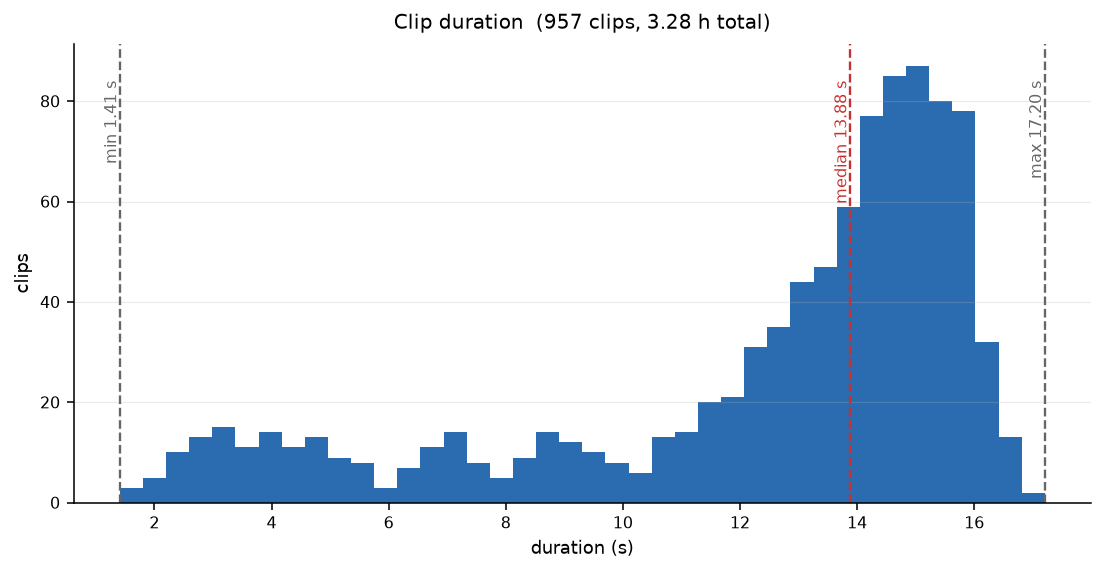
\includegraphics[width=1\linewidth]{durations.png}
    \label{fig:figure1}
    \vspace{0.8em}

    % Bottom figure
    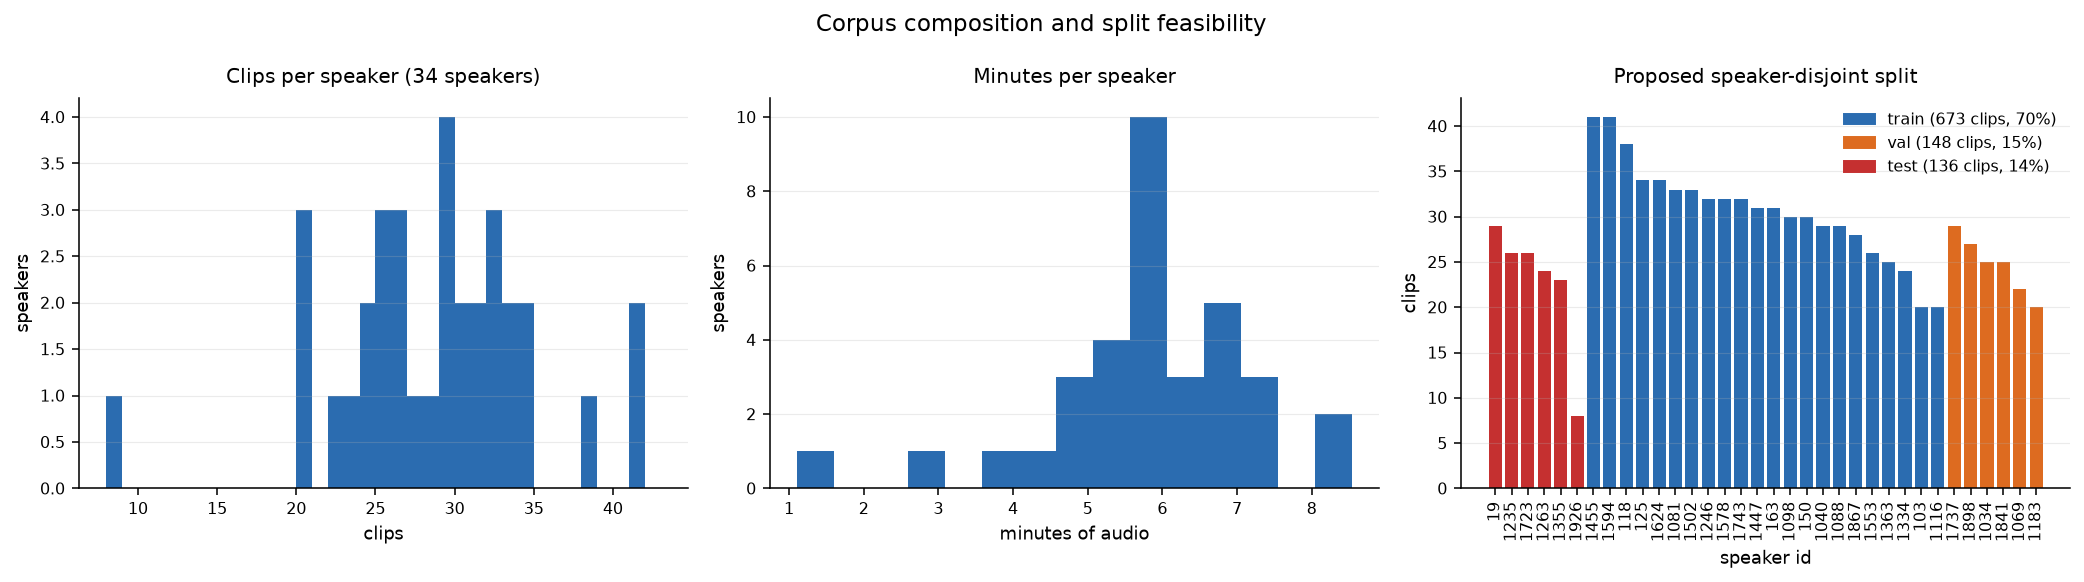
\includegraphics[width=1\linewidth]{speakers.png}
    \caption{Clips range from 1.4 to 17.2 s (median 13.9 s). Right: each speaker contributes 8 to 42 clips and 1 to 8 minutes; the corpus is large enough to hold out whole speakers for a disjoint split (Sec~\ref{sec:setup})}
    \label{fig:fig1}
\end{figure}






\subsection{Labels are silver with two reasonable conventions}

We know that the labels are generated using forced alignment, so they are reliable but not true ground truth\footnote{LibriSpeech does not come with word-level or phoneme-level timestamps/alignment}. We therefore treat them as high-quality silver labels and validate their quality independently later in the analysis.

One important question is how to handle short pauses between words. We noticed that the forced alignment labels pauses as non-speech, but very short gaps can reasonably be considered part of continuous speech. 
A design question arises immediately: Whether a short pause should be bridged into continuous speech ?

We therefore kept two labeling conventions (Fig~\ref{fig:gaps}) and run some stats on the entire data to determine the most suitable threshold\footnote{to bridge small pauses as contineous speech}. The literal labels follow the alignment segments exactly, while the bridged labels merge non-speech gaps shorter than a chosen threshold.  


\begin{figure}[H]
    \centering
    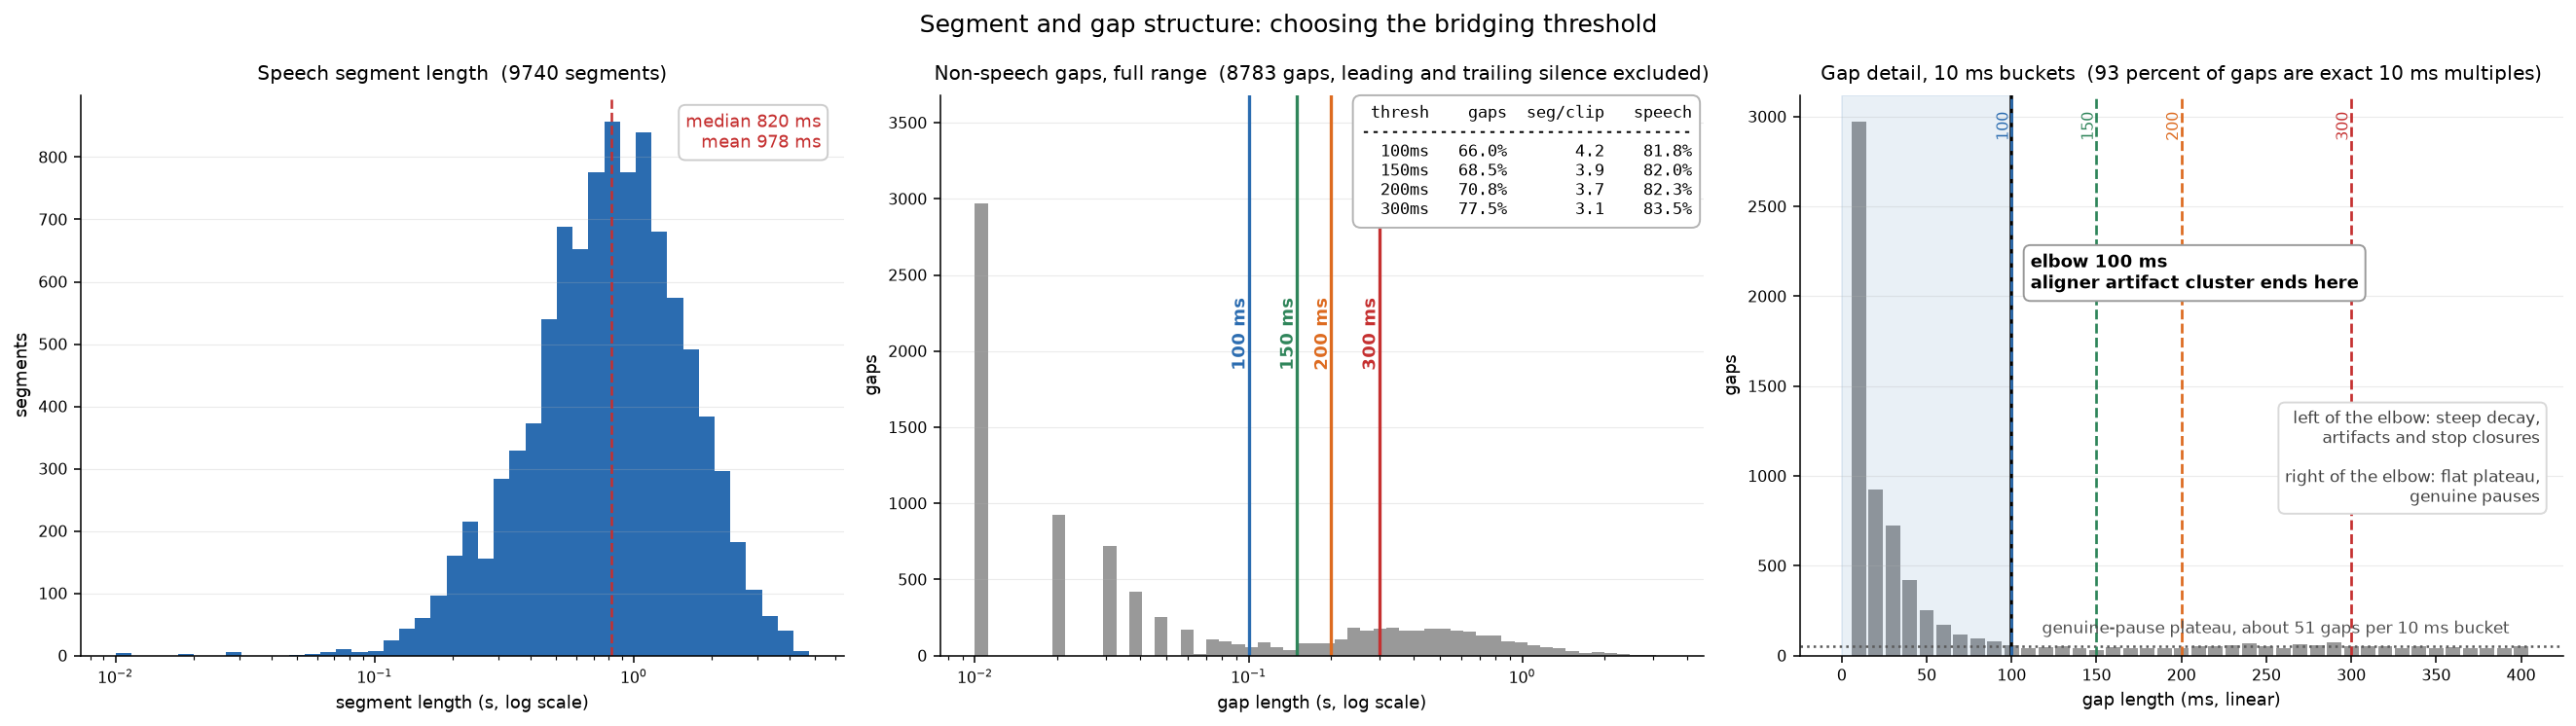
\includegraphics[width=1\linewidth]{segments_and_gaps.png}
    \caption{\textbf{Choosing the bridging threshold from the gap distribution.} The gap-length distribution is bimodal: a steep cluster of very short gaps below roughly 100 ms, then a flat plateau of genuine pauses above it. The short cluster is dominated by alignment artifacts and stop-closures (93\% of gaps are exact 10 ms multiples, the signature of frame-quantised alignment); the plateau is real inter-utterance pauses. We bridge at 100 ms, the elbow between the two regimes. This is a data-driven choice, not a tuned one, and the same 100 ms timescale reappears in the post-processing hangover (Sec~\ref{sec:post}).}
    \label{fig:gaps}
\end{figure}

\subsection{A low-frequency rumble justifies a high-pass front-end}

Listening to some audio clips from the datset and inspecting their spectrograms, we noticed energy concentrated below 80 Hz in labelled-silence regions of some clips. Speech has essentially no content below 80 Hz (Males start at 85Hz in general). This energy is therefore rumble, not signal, and it can mislead an energy-sensitive model into calling silence ``speech''.

We measure, for each clip, the fraction of total audio power below 80 Hz, both over the full recording and over forced-alignment silence frames, using an energy-weighted linear spectrogram statistic (Fig~\ref{fig:rumble}). We then flag high-rumble clips using the 90th percentile of the silence-only distribution (≈0.75), identifying recordings where low-frequency energy dominates during silence. 
After 96 clips (10\%) have more than 75\% of their silence-frame energy below 80 Hz. \textbf{This motivates an 80 Hz high-pass as the first stage of the front-end}.

We also studied the effect of the high pass filter Fig~\ref{fig:snr}. Left: per-clip SNR before and after the 80 Hz high-pass. The corpus is clean: most clips sit well above 13 dB, and the high-pass moves 96 clips out of the low-SNR region (176 below a 13 dB gate as recorded, 80 after). Right: the SNR gain is concentrated in low-SNR clips, confirming that what the filter removes is rumble in the silence frames rather than broadband noise on the speech. The key downstream implication: this corpus is clean, so a model trained on it alone will not have learned to handle noise, which motivates Sec~\ref{sec:robust}.


For the high-pass filter, we used a smooth second-order Butterworth biquad with zero-phase filtering. 

\begin{figure}[H]
    \centering
    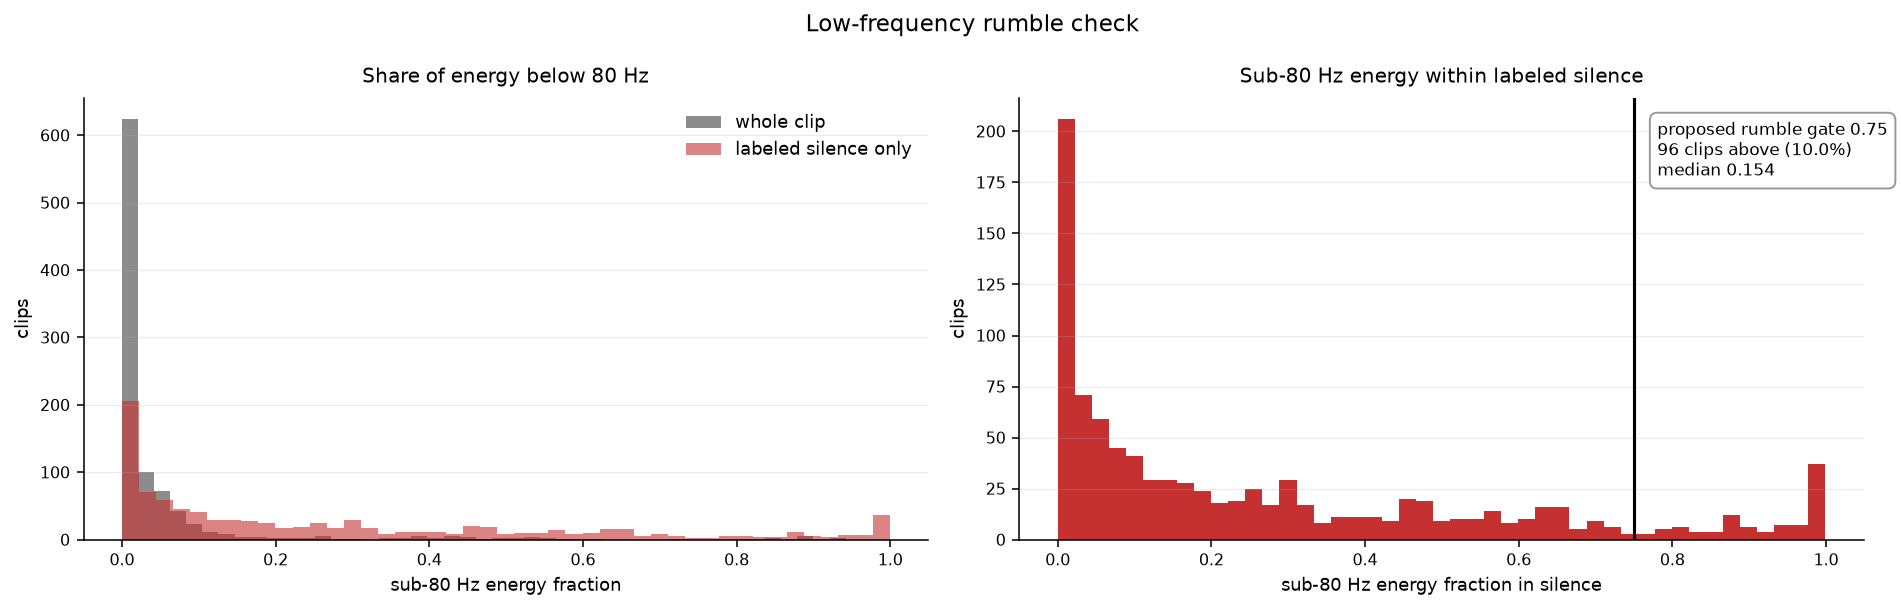
\includegraphics[width=1\linewidth]{rumble.png}
    \caption{\textbf{Low-frequency rumble check.} Silence frames carry disproportionate sub-80 Hz energy.}
    \label{fig:rumble}
\end{figure}

\begin{figure}[H]
    \centering
    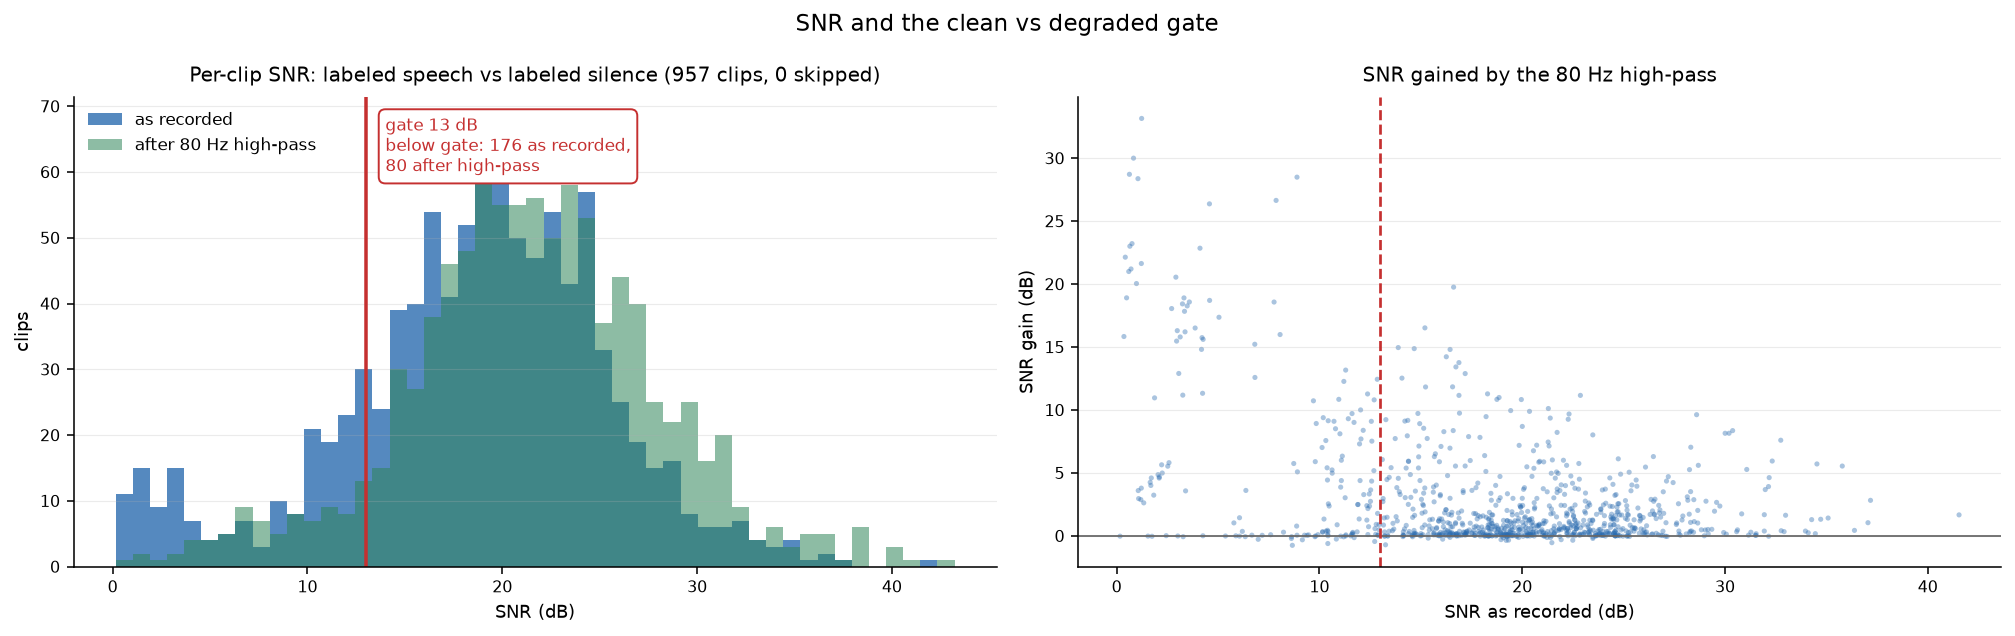
\includegraphics[width=1\linewidth]{snr.png}
    \caption{\textbf{SNR and the effect of the high-pass.}}
    \label{fig:snr}
\end{figure}

\begin{figure}[H]
    \centering
    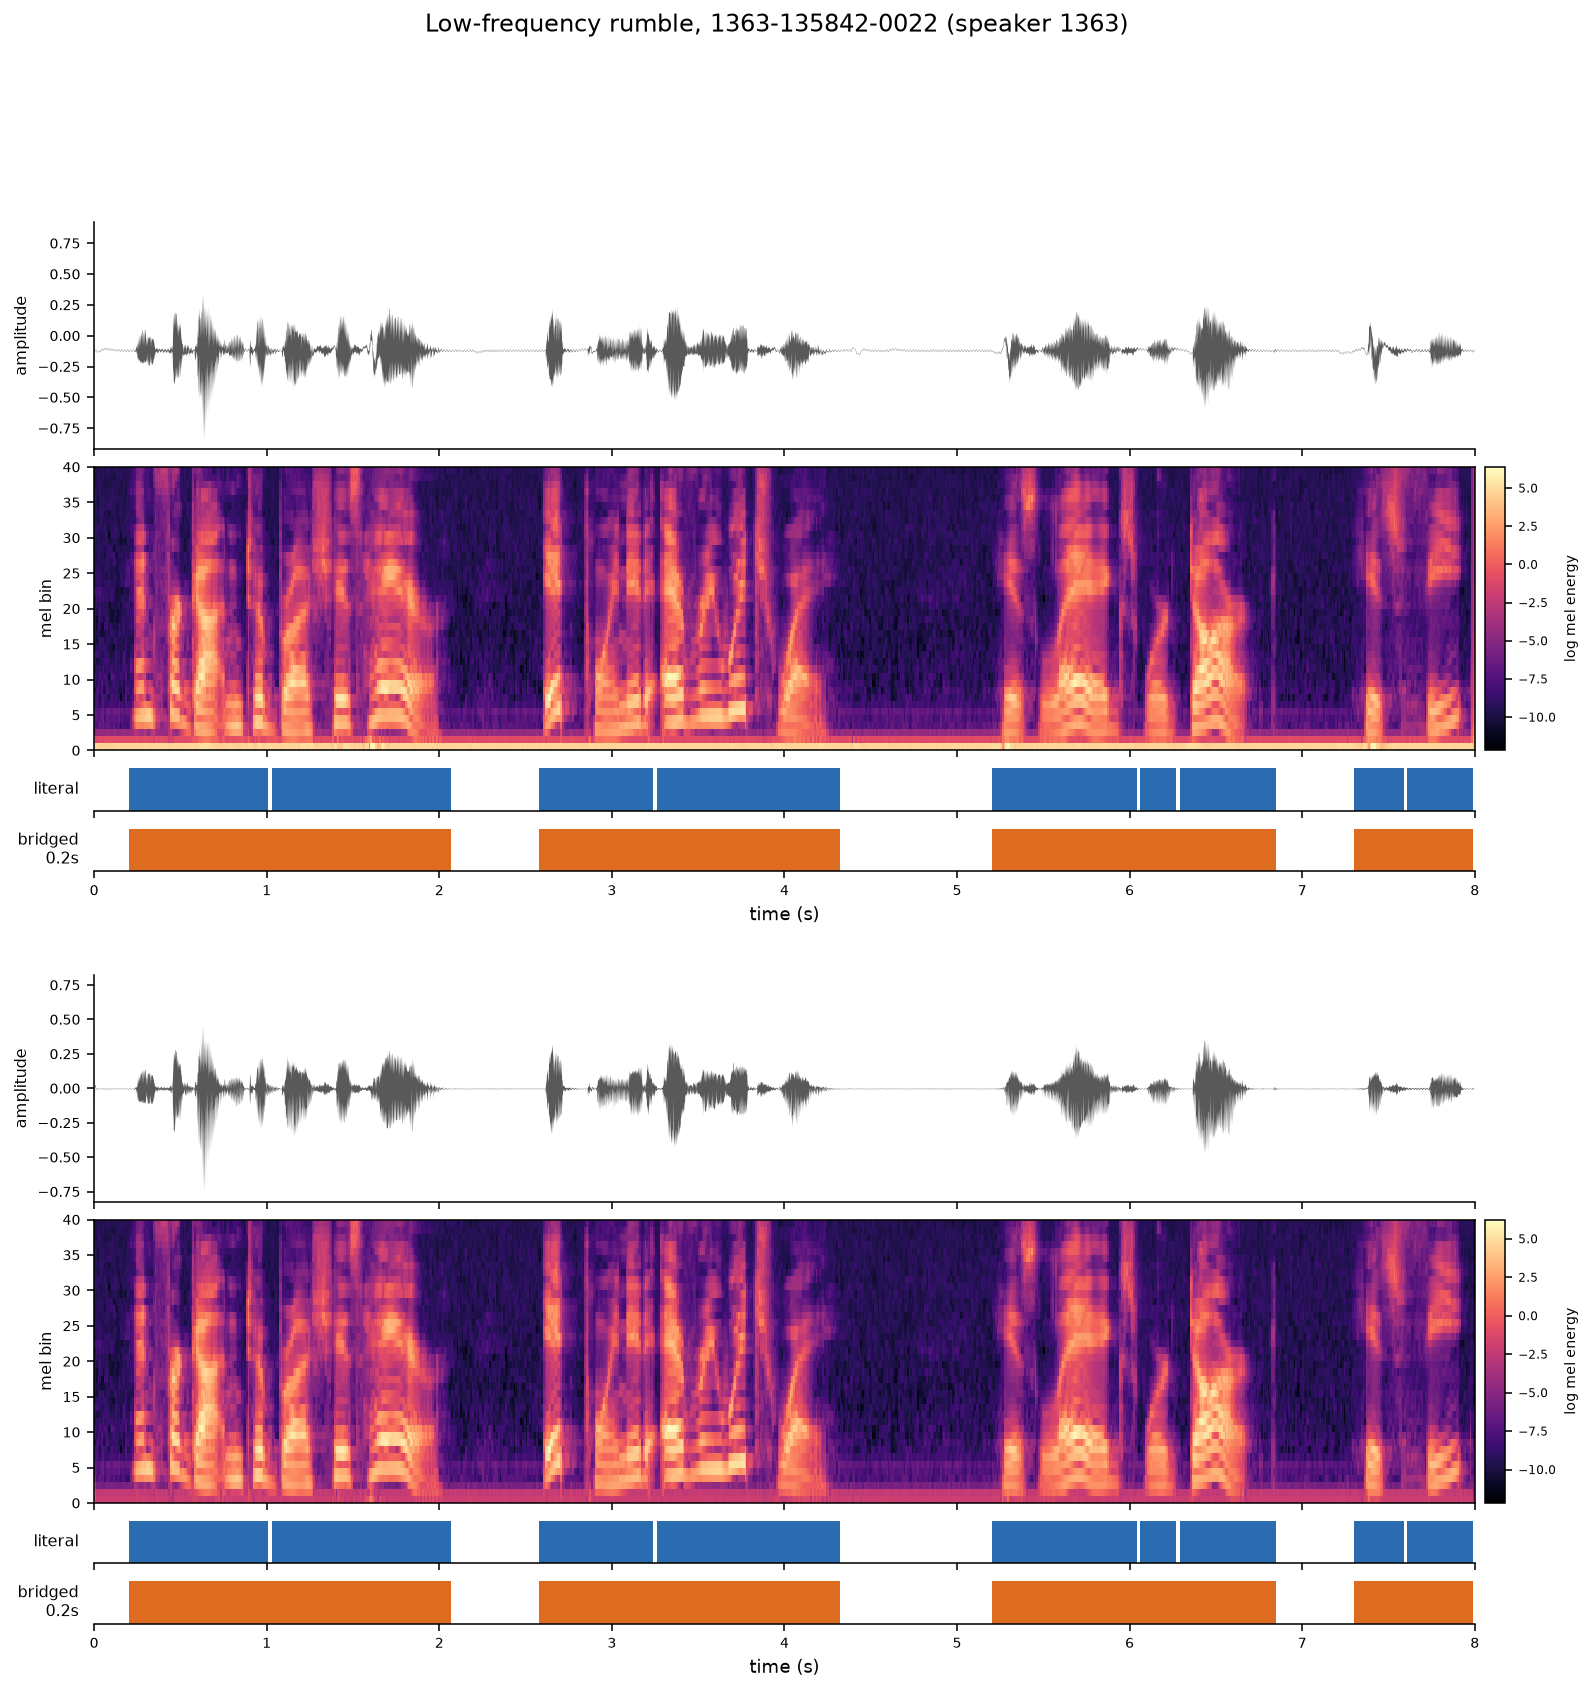
\includegraphics[width=1\linewidth]{rumble_highpass.png}
    \caption{\textbf{A representative clip after the 80 Hz high-pass, with both label conventions.} Visual overlays like this were our standard check that frame labels align with the acoustic content after every pipeline change.}
    \label{fig:highpass}
\end{figure}




\subsection{Position is not a shortcut}

A model can score well for the wrong reason. If speech were concentrated in a predictable part of each clip, the model could learn position instead of acoustics. We therefore measured the speech probability as a function of normalised position in the clip Fig~\ref{fig:position}. Speech is close to uniform through the body of the clip (mean 80.4\%), with only short silent margins at the edges. Position carries almost no information, so the model cannot exploit it as a shortcut; it must actually detect speech.

\begin{figure}[H]
    \centering
    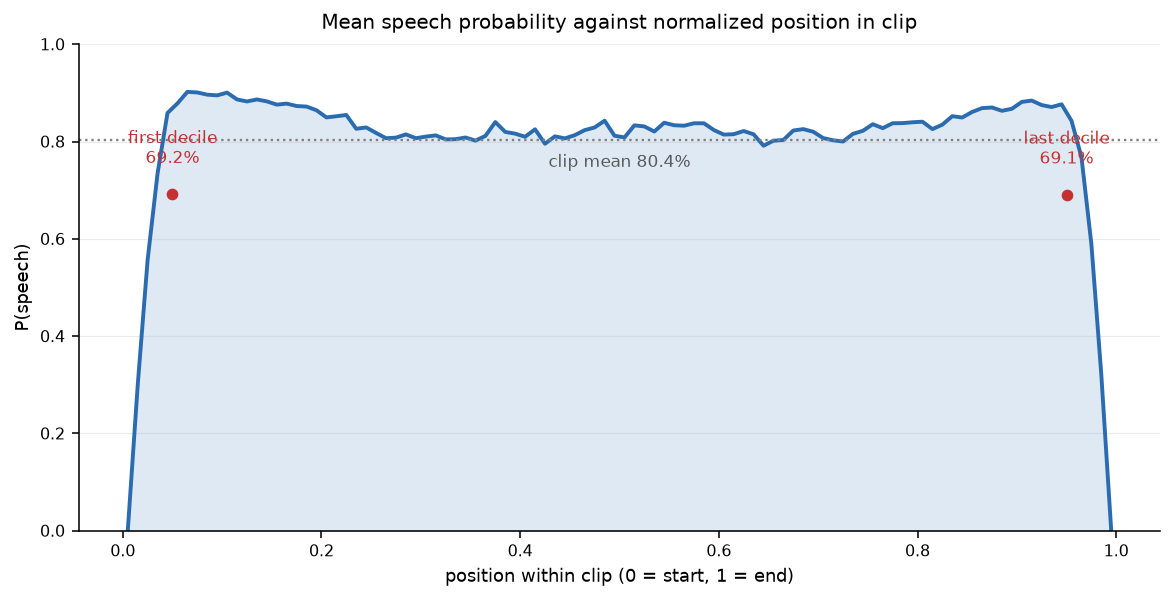
\includegraphics[width=1\linewidth]{position.png}
    \caption{\textbf{Speech probability against normalised position.} }
    \label{fig:position}
\end{figure}

\subsection{Independent validation of the labels}

To decide whether the silver labels are trustworthy \footnote{Mostely to check if you have introduced some bad clips on purpose}, we cross-checked them against Silero VAD Fig~\ref{fig:sileroagree}. Silero is an independent pretrained neural VAD trained on entirely different data, so its agreement with the aligner is not circular. Median per-clip speech-class IoU is 0.936 (literal) and 0.945 (bridged); median F1 is 0.967 and 0.972. No clip falls below 0.7 against either convention, so no clip is excluded. An independent model agrees with the labels on about 94\% of frames, so the labels are trustworthy. And bridged agrees better than literal, independent corroboration of the 100 ms bridging choice. \textbf{This motivate more to consider bridged pauses for the rest of the project}. 

 We pushed the study further to understand from where the residual disagreement comes from Fig\ref{fig:sileroboundary}. Silero places onsets a median $+45$ ms and offsets $+30$ ms later than the aligner, \textbf{the expected signature of a causal streaming VAD that needs a few frames of evidence before committing}. Almost all of the apparent disagreement is this boundary latency, not genuine conflict over where speech is. These numbers are important to keep in mind, as they will inform some of the design decisions we will need to make later for our streaming model.




\begin{figure}[H]
    \centering
    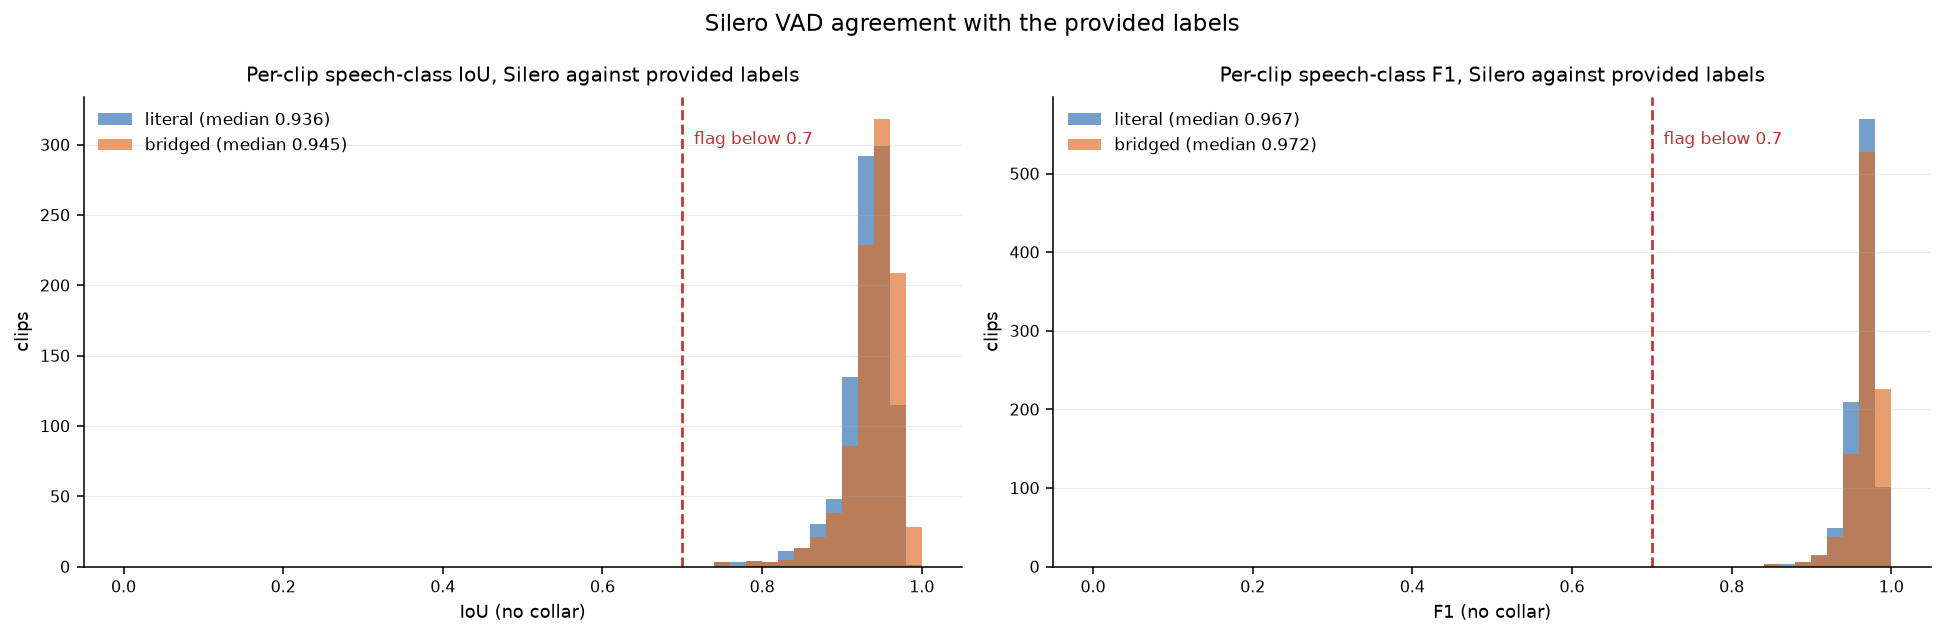
\includegraphics[width=1\linewidth]{silero_agreement.png}
    \caption{\textbf{Silero agreement with the provided labels.} }
    \label{fig:sileroagree}
\end{figure}

\begin{figure}[H]
    \centering
    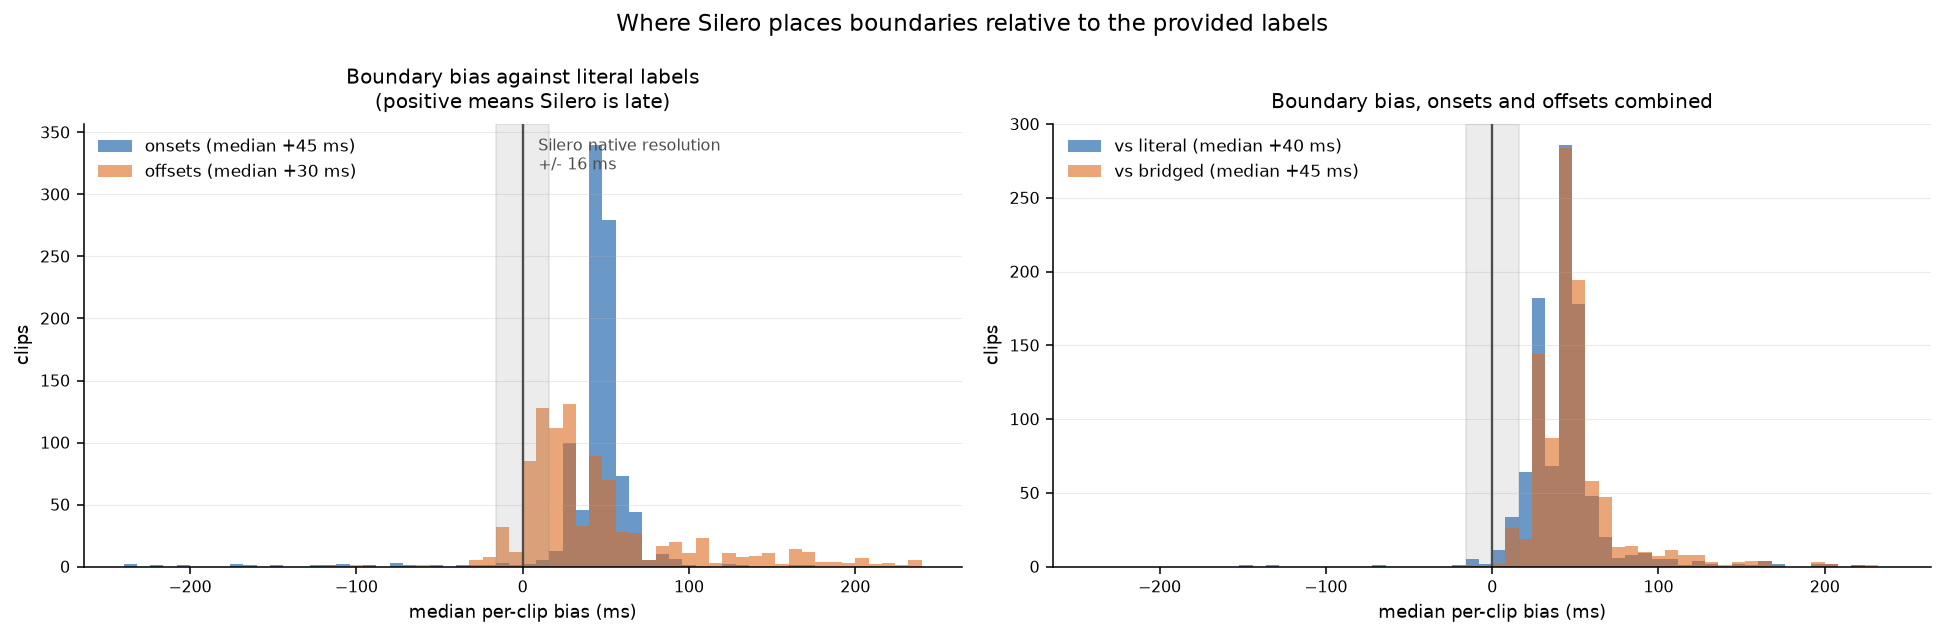
\includegraphics[width=1\linewidth]{silero_boundary_bias.png}
    \caption{\textbf{Where the residual disagreement comes from.}}
    \label{fig:sileroboundary}
\end{figure}

\subsection{Decisions carried into modelling}

The data analysis fixes three choices and one expectation. 
\begin{itemize}
\item (1) An 80 Hz zero-phase high-pass as the first front-end stage. 
\item (2) Labels at a 100 ms bridge, with literal retained for a sensitivity check. 
\item (3) A speaker-disjoint split. And the overarching finding that the corpus is clean, which predicts noise fragility and sets up the robustness study of Sec~\ref{sec:robust}.


\end{itemize}


\section{Experimental setup}
\label{sec:setup}

\paragraph{Speaker-disjoint split.} The 34 speakers are partitioned into 673 / 148 / 136 clips (roughly 70 / 15 / 15\%) with no speaker in more than one partition. LibriSpeech speakers are highly identifiable, so any overlap between train and test would let the model recognise the voice rather than detect speech, inflating every metric. Disjointness is enforced by construction and checked by a unit test. The noisier speakers were deliberately kept in training: the hard test conditions come from controlled augmentation (Sec~\ref{sec:robust}), not from whatever natural degradation falls in the test set.

\paragraph{Front-end.} Every clip passes the 80 Hz high-pass, then 40-band log-mel features at a 25 ms window and 10 ms hop (100 frames per second as shown in Fig~\ref{fig:framing}). Features are standardised with statistics computed on the training partition only and applied unchanged to validation and test, so no test-set scale information leaks into normalization.

\begin{figure}[H]
    \centering
    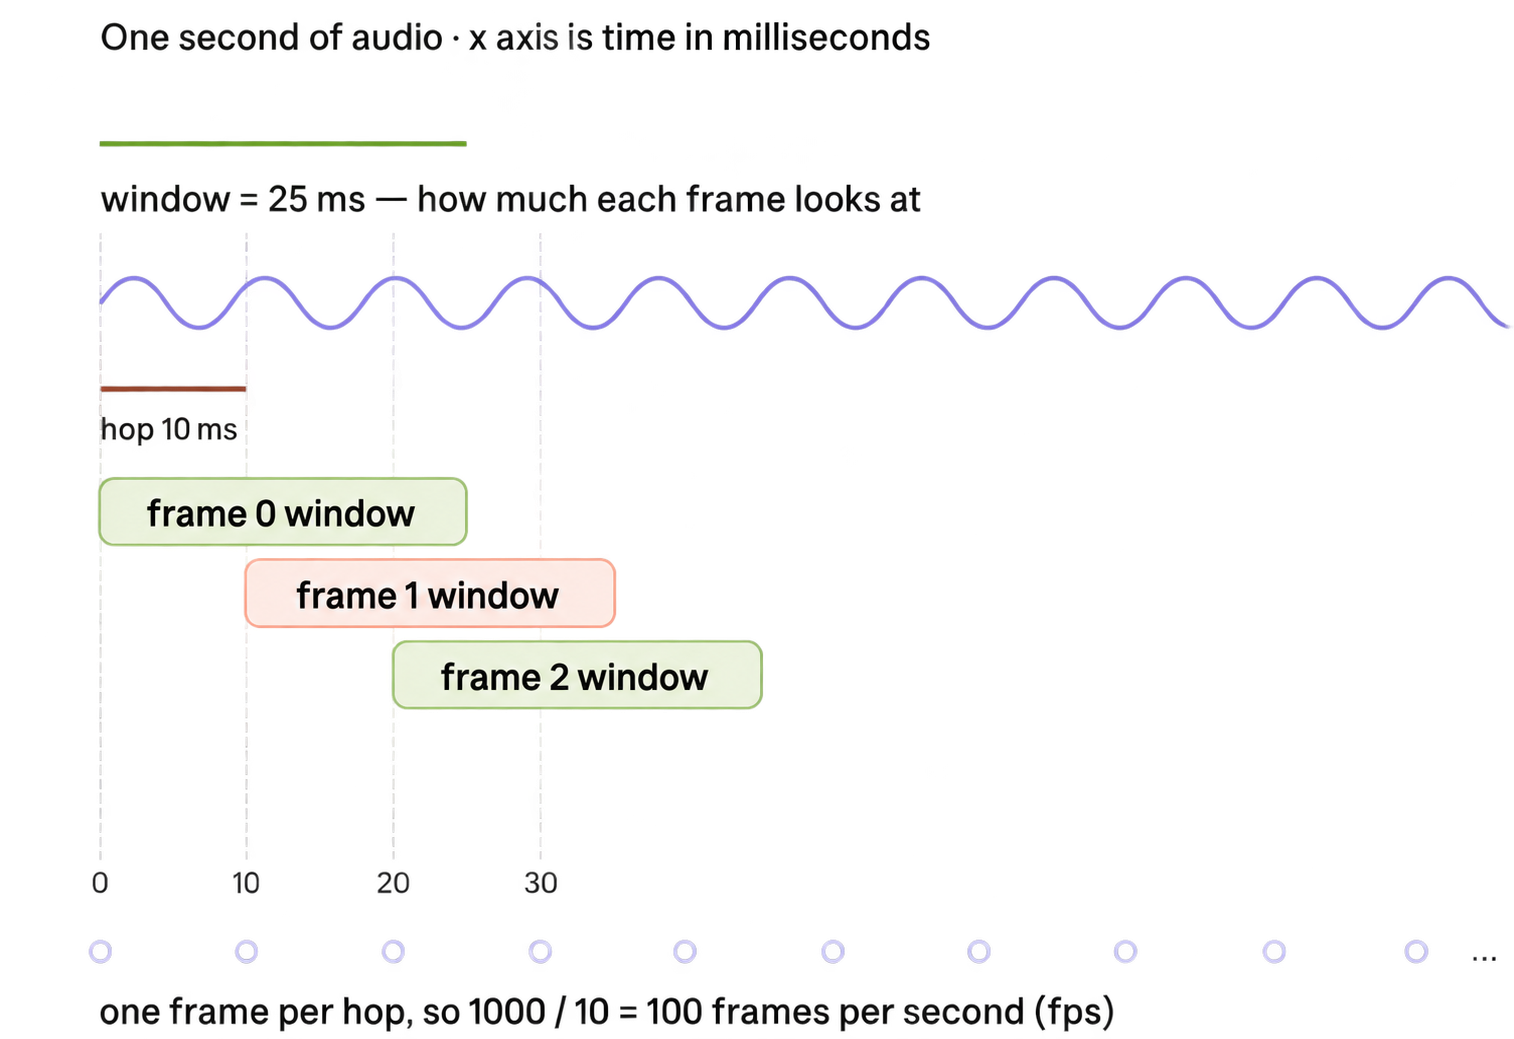
\includegraphics[width=0.92\linewidth]{framing.png}
    \caption{\textbf{The frame grid.} A 25\,ms analysis window advances by a 10\,ms hop, so
    consecutive windows overlap by 15\,ms and the frame rate is $1000/10 = 100$\,fps. Labels
    are rasterised on the \emph{hop} grid, not the window: frame $i$ owns
    $[i/100, (i{+}1)/100)$, so frames tile the clip exactly once and every logit is aligned
    frame-for-frame with its label.}
    \label{fig:framing}
\end{figure}

\paragraph{Class balance and metrics.} We studied the speech/non speech balance (Fig~\ref{fig:classbalance}). The corpus is about 81\% speech, an imbalance of roughly 4:1. This is mild and needs a light touch, not resampling, which is inappropriate for sequence labelling anyway. We handle it with a weighted loss (Sec~\ref{sec:train}), imbalance-robust metrics, and an operating point chosen on a DET curve. The primary metrics are EER and ROC/PR-AUC, which are threshold-free and do not depend on the class ratio the way accuracy does.

A little recall for what each metric measures:
\begin{itemize}
\item \textbf{Accuracy}: fraction of frames classified correctly. It can be misleading when classes are imbalanced.
\item \textbf{ROC-AUC}: measures how well the model separates speech from non-speech across all thresholds. Higher is better.
\item \textbf{PR-AUC}: summarizes the precision-recall trade-off across thresholds and is especially useful with class imbalance.
\item \textbf{EER}: error rate at the threshold where the false-positive rate equals the false-negative rate. Lower is better.
\item \textbf{DET curve}: shows the trade-off between false positives and false negatives as the decision threshold changes.
\end{itemize}


\begin{figure}[H]
    \centering
    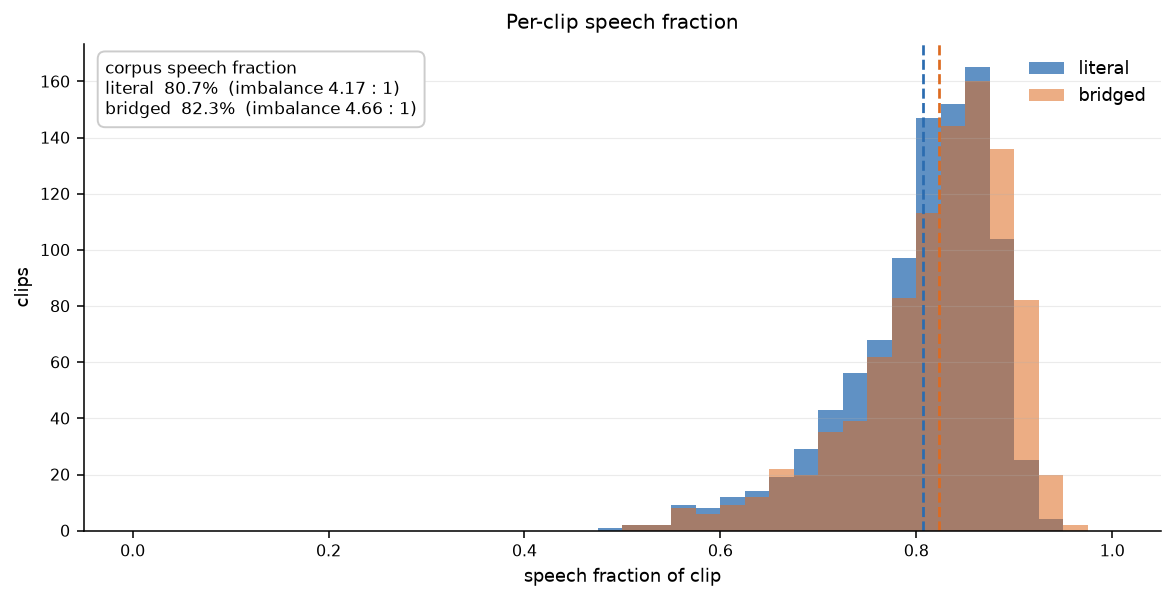
\includegraphics[width=1\linewidth]{class_balance.png}
    \caption{\textbf{Class balance.} Corpus speech fraction is 80.7\% (literal) and 82.3\% (bridged), an imbalance of 4.17:1 and 4.66:1.}
    \label{fig:classbalance}
\end{figure}

\paragraph{Threshold discipline.} Any threshold used to report an operating point is chosen on the validation split and applied unchanged to test. Threshold-free metrics are computed on test directly. No number in this report was tuned on test. Two distinct threshold families appear in the results, serving two objectives; they are kept separate and labelled (Sec~\ref{sec:thresholds}).

\section{Model architecture}
\label{sec:model}

\subsection{Architecture}

The detector operates at the frame level: for a sequence of log-mel feature frames it
emits one speech/non-speech logit per frame, trained against frame labels with binary
cross-entropy computed over valid (non-padded) frames only. The network factorises into
three parts: 

\begin{itemize}

\item A shared convolutional frontend mapping log-mel features to a per-frame
embedding of dimension $d_{\text{model}}$. and it is a known fact that such layer 
capture local dependencies.  

\item A temporal core that contextualises each frame
against its neighbours; 

\item A shared per-frame head, a layer normalisation followed by a linear projection to a single logit.

\end{itemize}
    
The frontend applies stride-1 convolutions in time and pools only along the mel axis, so
temporal resolution is preserved end to end and every output logit is aligned
frame-for-frame with its label (Fig~\ref{fig:framing}). The frontend and head are
identical modules across all experiments; only the temporal core is exchanged. This
isolation is deliberate: any difference in accuracy between cores is attributable to the
temporal model alone, with no confound from a differently-sized frontend or head.

We consider two cores. The first is a bidirectional GRU (Fig~\ref{fig:archbigru}), used as
an offline upper-bound baseline: it consumes the entire clip in both directions and
therefore cannot (not recommended) stream. The second is a causal masked-attention stack
(Fig~\ref{fig:archcausal}), the deployable streaming model that is the focus of this work.
Both cores return a tensor of the same shape, so the head is shared unchanged. Both models with shapes layer by layer are givven in Fig\ref{fig:archbigru}. 

\begin{figure}[H]
    \centering
    \begin{minipage}{0.48\linewidth}
        \centering
        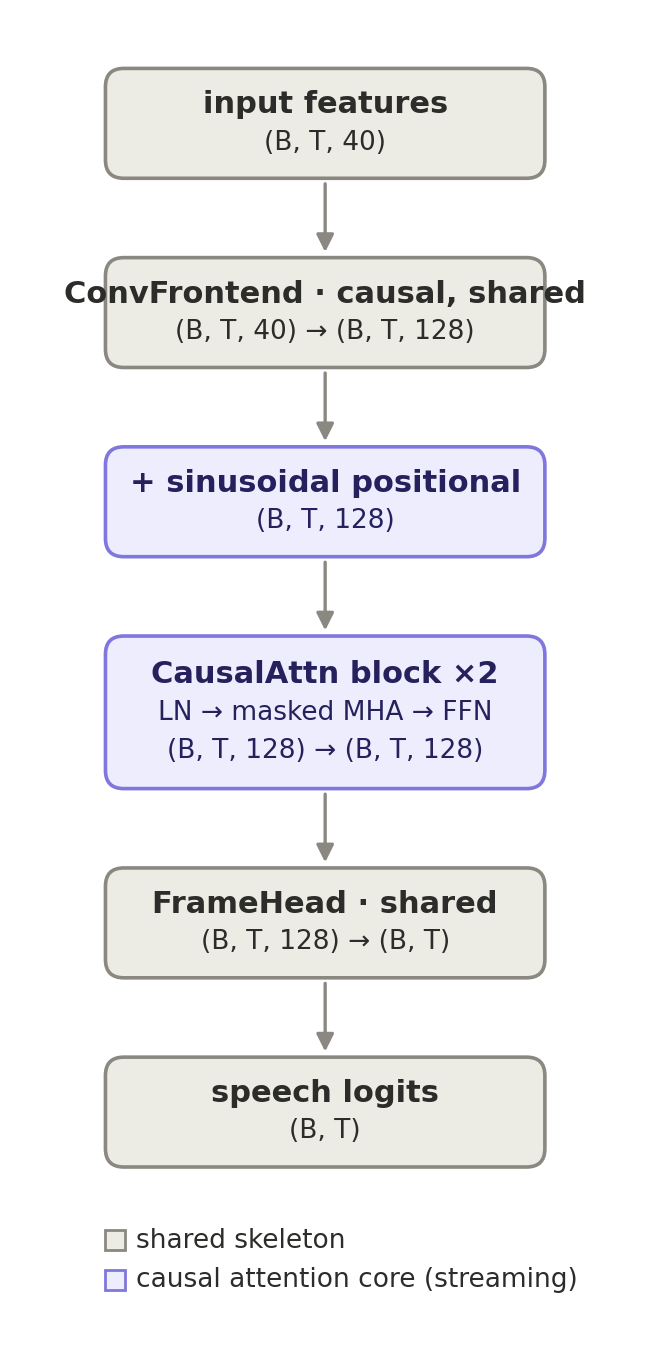
\includegraphics[width=\linewidth]{arch_causal.png}
    \end{minipage}\hfill
    \begin{minipage}{0.48\linewidth}
        \centering
        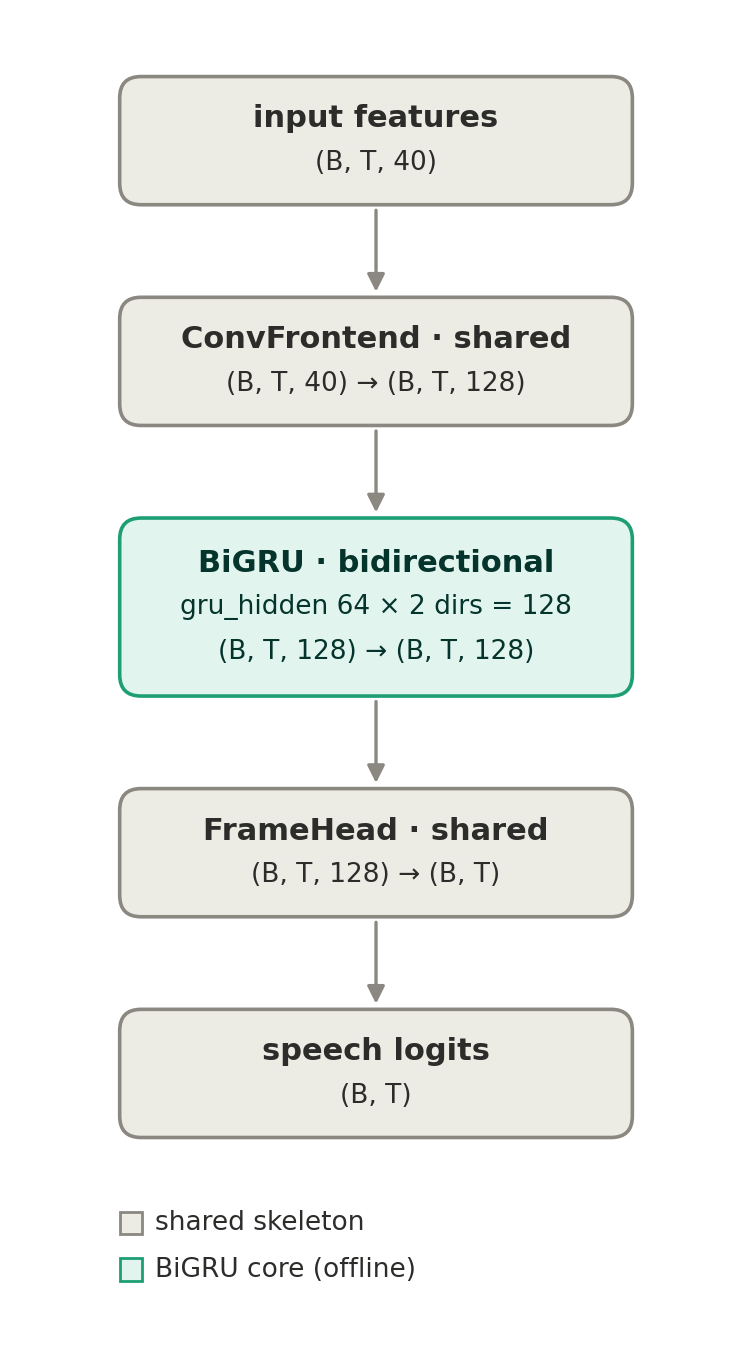
\includegraphics[width=\linewidth]{arch_bigru.png}
    \end{minipage}
    \caption{\textbf{One skeleton, two cores.} Left: the streaming causal-attention model.
    Right: the offline BiGRU. The convolutional frontend and the per-frame head are the
    same modules in both, so the accuracy gap in Sec~\ref{sec:clean} is attributable to the
    core alone. The BiGRU's $2\times64=128$ output already matches $d_{\text{model}}$, so no
    projection layer is needed between the core and the head. Shapes are those of the
    trained checkpoints. Let it be known that the number of heads is equal to 4 (four of the two attention layers)}
    \label{fig:archcausal}
    \label{fig:archbigru}
\end{figure}

\subsection{Causal masking: the training--deployment contract}

The attention core is made streaming-capable through a masked self-attention formulation.
For a query at frame $i$, attention to a key at frame $j$ is permitted only when
\[
    -W \;\le\; (j - i) \;\le\; L,
\]
where $W$ (\texttt{past\_window}) bounds how far back a frame may look and $L$
(\texttt{lookahead}) how far forward. $L=0$ yields a strictly causal model; $L>0$ admits a
bounded amount of future context per layer. This causal-window mask is combined with a
key-padding mask that forbids attention to the padded frames introduced when clips of
unequal length are batched together. The bounded past-context mechanism is inspired by the Sliding Window Attention used in Mistral 7B, while the optional lookahead is an extension specific to our streaming setting.

The two masks serve different purposes. The key-padding mask is a correctness requirement:
without it a real frame could attend to padding, making its output depend on how clips
happened to be grouped into a batch. Such a leak is invisible at evaluation time
(batch-norm statistics are frozen and dropout is disabled) and therefore easy to ship
unnoticed. The causal-window mask encodes the deployment contract, and this is the central
motivation for applying it during training rather than only at inference.

A streaming deployment can, by construction, only ever access a bounded window of past and
future frames. If the model were trained with unbounded attention, each frame free to attend to the whole clip, it would learn to rely on context that is simply unavailable
once the window is imposed at deployment. Restricting attention only at inference time
would then degrade accuracy, because the model is denied information it was trained to
use. We avoid this train--deploy mismatch by applying the identical mask in the single
masked forward pass used for both training and evaluation. Gradients therefore flow only
through the frame-to-frame connections that will exist at deployment, and the model learns
to make each decision from exactly the context it will have. The sweep in
Sec~\ref{sec:stream} shows this is not a theoretical concern: the unbounded-attention model
is the \emph{worst} configuration on the selection metric. 

Because the model is non-autoregressive, a batched forward pass carrying this window computes per-frame logits that are numerically identical to those of a true frame-by-frame streaming loop. Evaluation is therefore performed with the windowed batch forward, and the streaming implementation is retained only to verify this equivalence and to measure real per-frame latency and constant memory; the streamed and batched results are one and the same.

\begin{figure}[H]
    \centering
    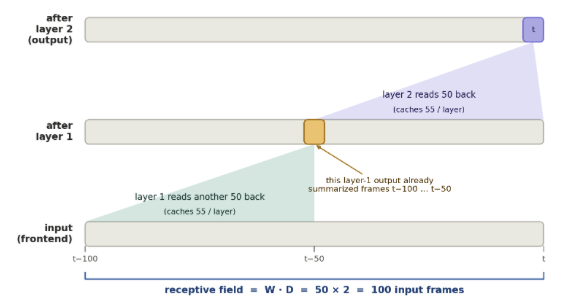
\includegraphics[width=0.92\linewidth]{receptive_field.png}
    \caption{\textbf{Why the per-layer window is not the deployed window.} The output at
    frame $t$ attends 50 frames back over the \emph{layer-1} sequence, but each of those
    layer-1 vectors had already summarised 50 frames of its own input, so the composed past
    reach is $W\!\cdot\!D = 100$ frames of frontend output. The cache is a separate
    quantity: it holds $W+L=55$ entries per layer, not 100. Measured end to end over raw
    log-mel input the past reach is 106 frames, the extra 6 coming from the causal
    convolutional frontend; the figure shows the attention composition alone.}
    \label{fig:receptive}
\end{figure}

One consequence of stacking attention layers is worth stating for latency accounting: the
per-layer window composes with depth. With $D$ attention layers, a frame's output
ultimately depends on frames up to $W\!\cdot\!D$ in the past and $L\!\cdot\!D$ in the
future (Fig~\ref{fig:receptive}). The effective context and the emission latency are both these composed figures, not the per-layer values.

\paragraph{The causal frontend, and why it is shared.} A symmetric convolution frontend
peeks a few frames into the future, which would make a ``strictly causal'' attention model
not actually causal. To keep the frontend genuinely shared and the streaming claim honest,
the frontend is causal for both cores. This costs the offline BiGRU a negligible amount
(about 30\,ms of local future context that its backward recurrence supplies anyway) and
keeps the core comparison clean. It also means the effective lookahead is exactly
$L\!\cdot\!D$, with no hidden contribution from the convolution stack.

\subsection{Operating point and scope}

The lookahead $L$ is the accuracy-versus-latency control of the model. We fixed a single
operating point rather than sweeping \footnote{Time constraint} it: the model was trained and deployed with a
per-layer lookahead of $L=5$ frames over $D=2$ layers, giving an effective future context
of $L\!\cdot\!D\!\cdot\!\tau = 100$\,ms at the 10\,ms frame hop $\tau$. Crucially, the same
lookahead is used at training and at deployment, in keeping with the contract above; the
past window $W$ is likewise bounded and matched between the two, so the deployed model
streams at constant memory. \footnote{In retrospect, I should have evaluated a smaller per-layer lookahead. My initial choice was based on the local lookahead of each attention layer, whereas the end-to-end future receptive field accumulates across the two stacked layers, yielding up to 100,ms of emission latency. This is an important distinction I would account for explicitly in a production iteration.}


A full latency/accuracy sweep over $L$, including the strictly causal $L=0$ point that uses no future context at all, would characterise the trade-off more completely, but was
out of scope for this task. The implementation parametrises $L$ directly, so evaluating an
alternative operating point, including a zero-lookahead minimum-latency deployment,
requires only a configuration change and a retrain, with no modification to the model or
the streaming code.

\subsection{Parameter budget}

\begin{table}[H]
    \centering
    \caption{Parameter budget. The frontend and the head are identical across the two
    models; only the temporal core changes, which is what makes the comparison in
    Sec~\ref{sec:clean} attributable to the core alone. Counts are read from the models
    the runs actually built, not from the configuration.}
    \label{tab:params}
    \small
    \begin{tabular}{lrr}
        \toprule
        Component & Offline (BiGRU) & Streaming (causal attention) \\
        \midrule
        Conv frontend (shared) & 97{,}152 & 97{,}152 \\
        Temporal core          & 148{,}992 & 264{,}960 \\
        Frame head (shared)    & 385 & 385 \\
        \midrule
        Total                  & 246{,}529 & 362{,}497 \\
        \bottomrule
    \end{tabular}
\end{table}

Table~\ref{tab:params} makes the split concrete. The frontend is 39\% of the offline
model and 27\% of the streaming one, and the head is 385 parameters, a layer norm and a
linear projection to a single logit. Everything that differs between the two is the
149k against 265k in the middle.

\paragraph{The context numbers, and why they are not the per-layer ones.} The deployed
streaming model sets 50 past frames and 5 lookahead frames \emph{per layer}, and stacks
two layers. By the composition above, the effective receptive field is twice the per-layer
figure in both directions: 100 frames of past, which is the 1\,s window
Sec~\ref{sec:stream} selects, and 10 frames of lookahead, which is the 100\,ms of model
latency itemised in Sec~\ref{sec:live}. That composition is the source of the third bug listed below, where the true lookahead was double what a single layer implied, and it is
why every window in this report is quoted as an effective value rather than a configured
one.

\paragraph{Testing caught three invisible issues.}
Discovering that the effective emission latency was twice what we had initially assumed prompted a deeper set of unit tests. These tests surfaced issues that can produce plausible-but-wrong results while leaving the training loss apparently normal. First, padded frames could leak through the convolutional stack: convolution and normalisation biases can create non-zero activations at padded positions, which a subsequent convolution may propagate back into the last valid frames. As a result, a clip's prediction could depend on the other clips in the same batch. Attention masking alone cannot prevent this, because the contamination occurs before the attention layers; a key-padding mask can ignore padded keys, but cannot repair an already corrupted valid representation. Second, batch normalisation could incorporate padded frames into its running statistics, an effect that is easy to miss when inspecting the model only in evaluation mode. Third, I found that per-layer attention lookahead composes across stacked layers, so two layers with the same lookahead yield twice the future receptive field implied by inspecting a single layer. Each issue is now covered by a dedicated unit test. The padding-leakage issue is additionally prevented by the committed configuration, which pads the frontend on the left only; therefore, it was latent rather than active in the reported runs.


\section{Training}
\label{sec:train}

Training uses a masked, weighted binary cross-entropy. The positive-class weight is the ratio of non-speech to speech frames computed on the training partition only (0.233 for bridged), which down-weights the majority speech class. Padded frames are excluded from the loss via the batch mask. We use AdamW, a learning-rate schedule, gradient clipping, fixed seeds, checkpoint selection on validation false-rejection at the false-alarm operating point (frr\_at\_fa), and early stopping. On an Apple M5 laptop (24GB) the offline model trains in about 150 s per epoch and converges within roughly ten epochs.

Weighting is a light adjustment, not the main lever. Because the operating point is chosen downstream on a DET curve, the exact weight mostly shifts where the untuned threshold sits and is absorbed by the threshold choice. We judged that focal loss is unnecessary at a 4:1 ratio, and resampling was rejected as
inappropriate for sequence labelling.

\paragraph{Measured cost, and what augmentation adds to it.} Every run was trained on an
Apple M5 laptop (24GB) through the MPS backend, at batch size 8 over the 673 training
clips. Table~\ref{tab:cost} gives the measurements, and two things in it are worth
reading.

\begin{table}[H]
    \centering
    \caption{Measured training cost. Every run was given the same 30-epoch budget with
    early-stopping patience 8, and every run finished: the three marked with an early stop
    ran out of patience, and the augmented offline model used the whole budget. Seconds per
    epoch are the training pass alone; validation adds about 8.5\,s per epoch for the
    offline model and 1.3\,s for the streaming one. ``Selected'' is the epoch the selection
    metric chose, which is the checkpoint every reported number comes from.}
    \label{tab:cost}
    \setlength{\tabcolsep}{5pt}
    \small
    \begin{tabular}{llrrrr}
        \toprule
        Model & Training & s\,/\,epoch & Epochs run & Selected & Wall clock \\
        \midrule
        Offline BiGRU & clean     & 142.7 & 16 (early stop) & 8  & 40m 19s \\
        Offline BiGRU & augmented & 167.7 & 30 (full budget) & 22 & 88m 04s \\
        Causal 1\,s   & clean     & 24.3  & 16 (early stop) & 8  & 6m 51s \\
        Causal 1\,s   & augmented & 48.6  & 28 (early stop) & 20 & 23m 19s \\
        \bottomrule
    \end{tabular}
\end{table}

The first is that the streaming model is much the cheaper one to train, 24.3\,s per epoch against 142.7\,s on clean data and a factor of 5.9, despite carrying 47\% more
parameters (Table~\ref{tab:params}). A bidirectional recurrence is sequential in the
frame index and cannot use the accelerator's width; masked attention over a bounded
window is a batched matrix product. Parameter count is a poor predictor of training cost
here: the streaming model is at once the cheaper to train and the only one of the two
that can run on a live stream, and it pays for both only in accuracy.

The second is that augmentation costs a flat 25\,s per epoch: $+25.0$\,s for the offline
model and $+24.3$\,s for the streaming one, about 36\,ms per clip. The two increments
match because the work is the same in both cases and happens in the same place: the dataloader runs in the main process, ahead of whichever core is training, and the
augmented dataset cannot cache its features, since the point is a fresh room and a fresh
interferer every epoch. That is why the same absolute cost reads as 17\% on the offline
model's epoch and as a doubling of the streaming model's.

Augmentation also needs more epochs, not merely longer ones. Both clean runs select
epoch 8 and then early-stop at 16, having spent the full patience without improving; both
augmented runs select much later, epoch 22 for the offline model and epoch 20 for the
streaming one. A wider training distribution is simply a harder fit. The clean runs are
the evidence that the budget was adequate on both sides: they were given the same 30
epochs as the augmented runs and declined to use them.

\section{Results: clean performance}
\label{sec:clean}

On the held-out test speakers the offline model reaches 2.02\% EER and 0.9951 ROC-AUC, and it outperforms both reference VADs: a classical one (WebRTC) and a strong pretrained neural one (Silero). Table~\ref{tab:clean} reports the comparison.

\begin{table}[H]
    \centering
    \caption{Clean-test performance against the two reference VADs. Best value per column in bold.}
    \label{tab:clean}
    \setlength{\tabcolsep}{4pt}
    \small
    \begin{tabular}{lrrrp{1.9cm}}
        \toprule
        System (clean test) & EER $\downarrow$ & ROC-AUC $\uparrow$ & PR-AUC $\uparrow$ & Streamable \\
        \midrule
        Offline BiGRU (ours)           & \textbf{2.02\%} & \textbf{0.9951} & \textbf{0.9981} & no \\
        Causal attn., 1 s (ours)       & 2.47\%          & 0.9931          & 0.9977          & yes, constant memory \\
        Silero VAD                     & 6.18\%          & 0.9815          & 0.9953          & yes \\
        WebRTC VAD (mode 3)            & 6.97\%          & 0.9354          & 0.9821          & yes \\
        \bottomrule
    \end{tabular}
\end{table}

WebRTC emits binary decisions, so its ``EER'' is its single operating point. Mode 3 is the aggressiveness setting selected on validation; modes 0 to 2 are near-useless here (27 to 35\% EER).

\begin{figure}[H]
    \centering
    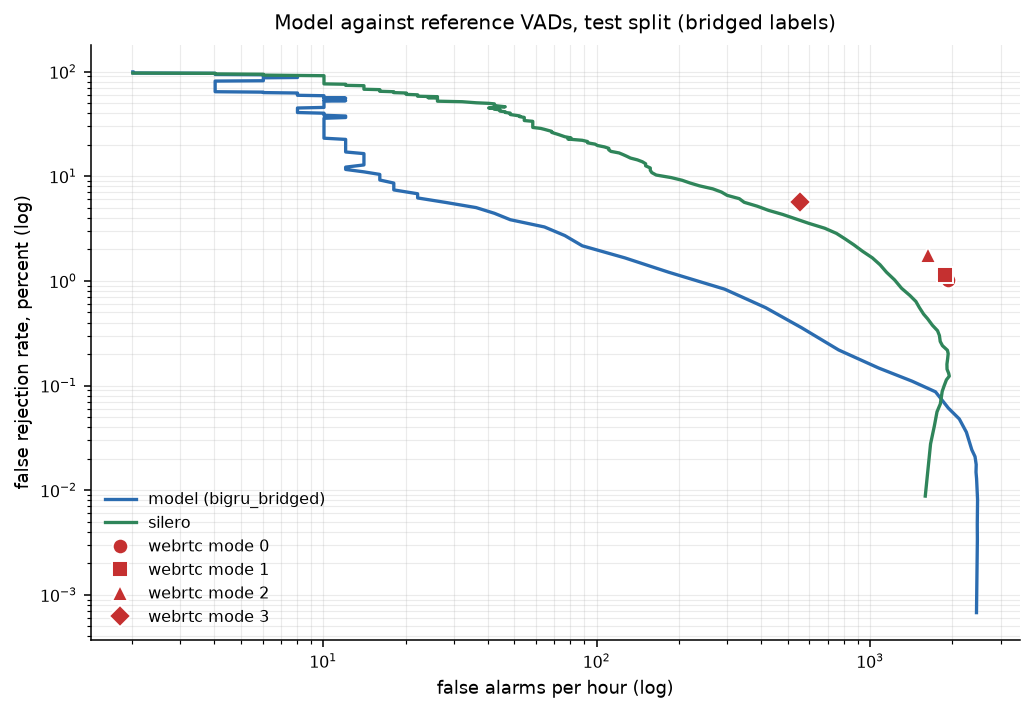
\includegraphics[width=1\linewidth]{baseline_det.png}
    \caption{\textbf{Detection error trade-off on the test set.} Lower and to the left is better. Our model (blue) sits below Silero (green) across essentially the entire operating range. WebRTC's four modes (red markers) sit far to the right at hundreds to thousands of false alarms per hour. The steep rise at the far left (below roughly 10 to 20 false alarms per hour) is a resolution artifact of the 0.5-hour test split, where the false-alarm budget permits only a few events; the comparison should be read from the body of the curve and from EER/AUC.}
    \label{fig:det}
\end{figure}

The honest framing is this. Silero is trained for robustness across more than 100 languages, whereas our model is trained for clean read English. The comparison shows a domain-matched model beating a general one on the target distribution, which is the expected result rather than a claim of a better model in general.

\section{The streaming model and its context}
\label{sec:stream}

The causal-attention model reaches 2.47\% EER, close to the offline BiGRU's 2.02\%, while being deployable on a live stream at constant memory. The gap is the price of causality: the offline model uses the entire future of the clip, which is exactly what forbids it from streaming.

How much past context does a streaming VAD need? VAD is a local decision, and the gap analysis in Sec~\ref{sec: data} suggested the informative timescale is sub-second. We swept the bounded past window over 0.5, 1, 2, and 4 seconds, using the same checkpoint-selection metric as training, validation false-rejection at the false-alarm operating point. Table~\ref{tab:sweep} gives the sweep.

\begin{table}[H]
    \centering
    \caption{Past-window sweep on the validation split. The selection metric is FRR at the false-alarm budget; best value per column in bold, and the worst selection-metric value marked $\dagger$. The 1 s window is selected.}
    \label{tab:sweep}
    \setlength{\tabcolsep}{3pt}
    \small
    \begin{tabular}{lrrrrr}
        \toprule
        Causal window & Best epoch & FRR at FA budget $\downarrow$ & FA/hour & EER $\downarrow$ & ROC-AUC $\uparrow$ \\
        \midrule
        0.5 s          & 4 & 7.40\%                     & 98.7 & 3.53\%          & 0.9904 \\
        \textbf{1 s}   & 8 & \textbf{6.25\%}            & 96.6 & 3.27\%          & 0.9899 \\
        2 s            & 8 & 7.43\%                     & 98.7 & \textbf{3.22\%} & 0.9902 \\
        4 s            & 6 & \textit{9.78\%}$^{\dagger}$& 94.5 & 3.87\%          & 0.9889 \\
        \midrule
        Unbounded      & 8 & 9.77\%                     & 96.6 & 3.78\%          & 0.9891 \\
        \bottomrule
    \end{tabular}
\end{table}

Validation split, bridged labels, lookahead 5 frames per layer. Windows are effective values, since they compose across the two attention layers.

The 1 s window is selected. On the stated selection criterion it achieves the lowest false-rejection (6.25\%), a roughly 16\% relative reduction over 0.5 s and 2 s at essentially the same 100-per-hour false-alarm operating point. The 2 s configuration reaches a marginally lower EER (3.22\% versus 3.27\%), but the difference is tiny while its operational false-rejection is meaningfully worse, so we did not choose 2 s on the strength of a 0.05-point EER edge. The sweep also gives a clean architectural conclusion: more context does not monotonically help. Performance peaks around 1 s, stays competitive at 2 s, and clearly deteriorates at 4 s. This suggests the model extracts what it needs from about one second of history, and that additional history adds little and may make attention less focused. Also the false-rejection at the false-alarm budget in shown Fig~\ref{fig:sweep} motivates further the 1s bounded window.

\begin{figure}[H]
    \centering
    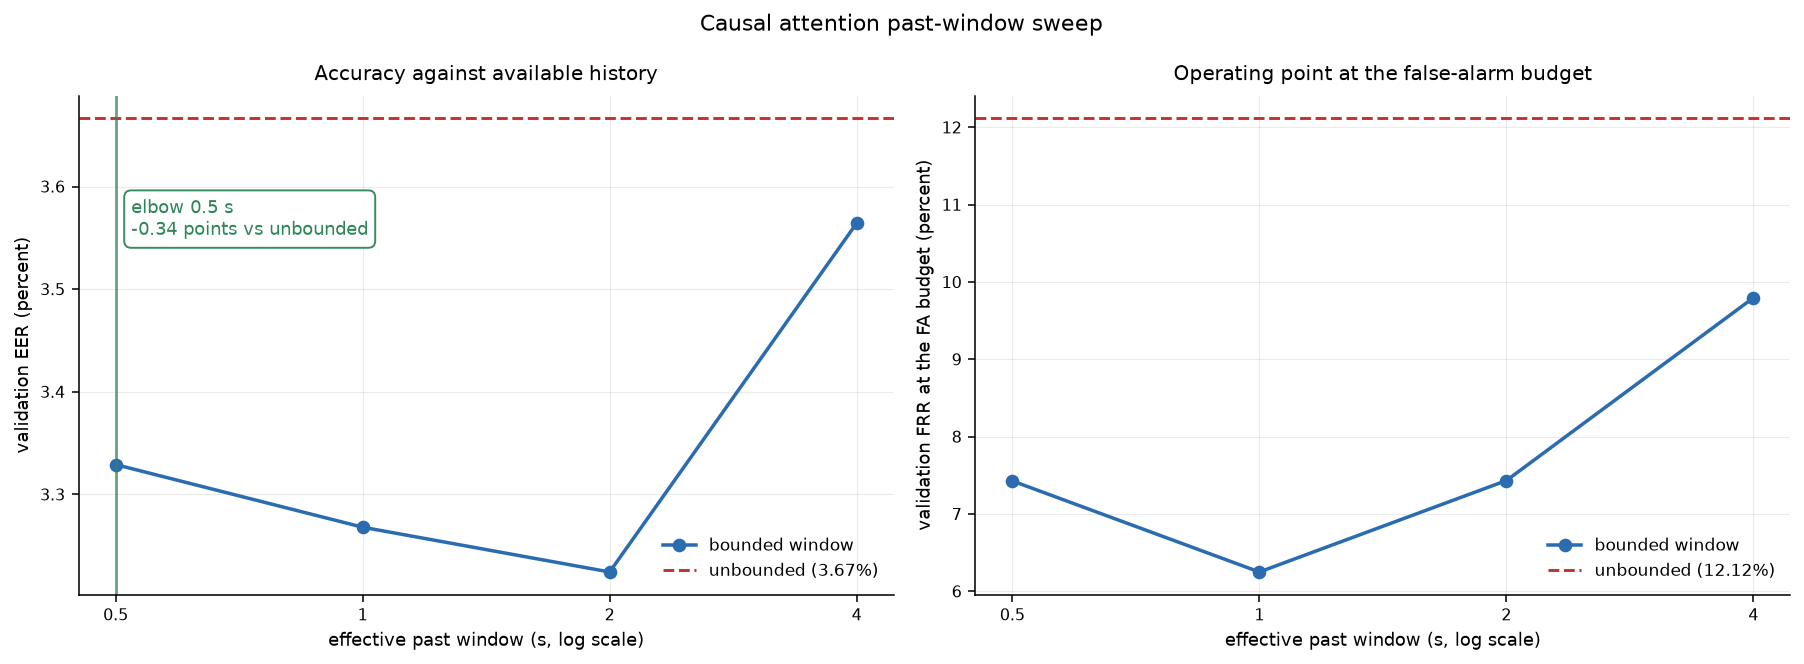
\includegraphics[width=1\linewidth]{past_window_sweep.png}
    \caption{\textbf{Accuracy against available past context, validation split.} Left: EER; right: false-rejection at the false-alarm budget, the selection metric. The right panel is the operative one and shows the minimum at 1 s.  Bounded windows up to 2 s beat unbounded attention (dashed) outright, and by 4 s the bounded model has simply converged to it (9.78\% against 9.77\%). A bounded window therefore gives constant-memory streaming at no accuracy cost, and the reason is that VAD's informative context is short: seeing the whole clip is not better than seeing the last second, it is worse.}
    \label{fig:sweep}
\end{figure}

\section{Streaming inference and caching}
\label{sec:cache}

\paragraph{Streaming as a windowed forward pass.} The model is non-autoregressive: a frame's logit is never fed back as input. Streaming is therefore not required to \emph{produce} our results. A batched forward pass carrying the same causal window
(Sec~\ref{sec:model}) computes per-frame logits that are numerically identical to a true
frame-by-frame loop, and all reported metrics use that windowed batch forward. Streaming is
instead the \emph{deployment} form of the same computation: at inference the model consumes
one frame at a time and must emit a logit under a fixed latency and a fixed memory budget,
regardless of how long the audio stream runs.

The bounded attention window from training is exactly what makes this possible. Each output
frame depends only on the frames inside its window, so the frames that scroll off the past
edge can never affect any future output. A naive implementation could therefore recompute
the window from scratch at every step and still be correct, but that cost grows with the
window and the network depth. The key-value cache removes that redundancy (inspired by llm inference).

\paragraph{The key--value cache.} Per attention layer, the cache retains the key and value
projections (and the intermediate representations) of the frames currently inside the
window. Each step performs three moves: \emph{project} the newly arrived frame once and
store its key/value; \emph{reuse} every frame still inside the window directly from the
cache, with no recomputation; and \emph{evict} any frame older than $i - W$, which has now
left the window and can influence no further output. Because the retained representations
are cached at every layer, the reuse holds throughout the depth of the network, not only at
the first layer. The consequence is that per-frame work is constant in the length of the
stream: at steady state each new frame triggers one projection per layer and an attention
over a fixed number of cached entries.

\begin{figure}[H]
    \centering
    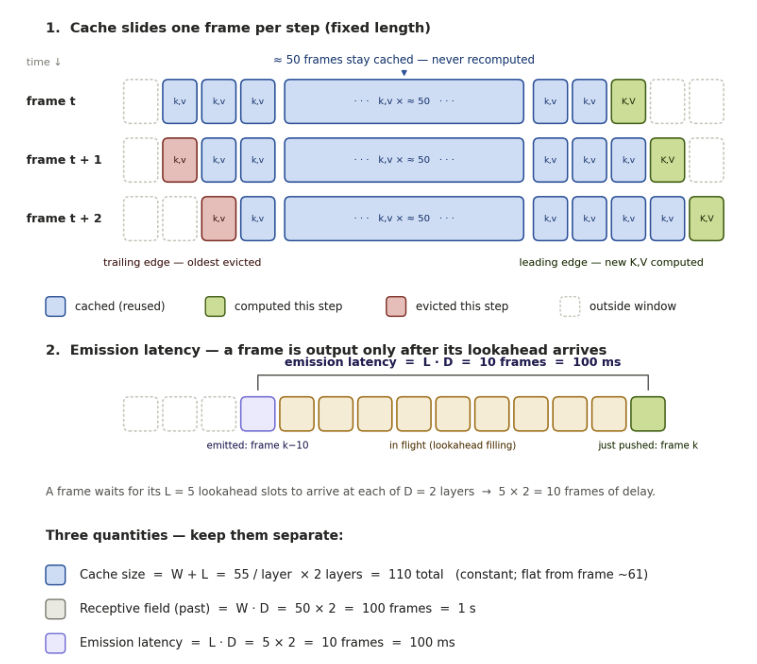
\includegraphics[width=\linewidth]{kv_cache_window.png}
    \caption{\textbf{Streaming cache, latency, and the three quantities.} \emph{Top:} three
    consecutive steps. Each computes one new key/value pair per layer at the leading edge,
    evicts the oldest at the trailing edge, and reuses the remaining 54 from the cache, so
    per-frame work and memory are constant in stream length; the loop advances one frame
    per step, not in 100\,ms chunks. \emph{Middle:} a frame is emitted only once its
    lookahead has arrived at every layer, so pushing frame $k$ releases frame $k-10$, verified in the live session, where 199 pushed frames had emitted up to frame 189.
    \emph{Bottom:} the three figures that are routinely conflated. Cache size $W+L=55$ per
    layer, 110 across both, flat from frame 61 onwards; past receptive field
    $W\!\cdot\!D=100$ frames; emission latency $L\!\cdot\!D=10$ frames.}
    \label{fig:kvcache}
\end{figure}

\paragraph{Constant memory.} Eviction is what bounds the memory. With a per-layer past
window $W$, lookahead $L$, and $D$ attention layers, the cache holds at most $W + L + 1$
entries per layer, each a key and a value vector of $d_{\text{model}}$ floats (the per-head
split $n_{\text{heads}} \times d_{\text{head}}$ equals $d_{\text{model}}$). The total cache
is therefore
\[
    C \;=\; (W + L + 1)\; D\; d_{\text{model}} \times 2 \quad \text{floats},
\]
plus a small frontend buffer of $\texttt{frontend\_context} + 1$ input frames. At the
deployed setting ($W=50$, $L=5$, $D=2$, $d_{\text{model}}=128$) this is 28{,}672 float32
values, or 112\,KiB. Every term is independent of the stream length, so the footprint is
identical for one second or one hour of audio; instrumenting the live session confirms the
resident set flattens after the first $W+L$ frames and does not move thereafter.

This constancy depends entirely on the finite past window. With an unbounded past the model
still produces correct logits, but the cache grows without bound as frames accumulate and
the configuration is not deployable in a streaming setting. Bounding $W$, and bounding it identically at training time per the training--deploy contract, is what converts the
model from offline to streamable.

\paragraph{Latency.} A frame cannot be finalised until its lookahead budget has been filled
at every layer, so the emission delay is $L\!\cdot\!D$ frames, that is $L\!\cdot\!D\!\cdot\!\tau$
for a frame hop $\tau$. That is 100\,ms here, the largest single term in the live latency
budget of Sec~\ref{sec:live}. A strictly causal configuration ($L=0$) emits with no added
delay. At the end of a stream the tail frames, which sit inside the lookahead delay, are
released against whatever future has actually arrived, the same behaviour the batch path
exhibits, where the padding mask blocks keys beyond the final frame.

\paragraph{Scope.} The positional encoding is absolute, so while the cache size is constant,
the position indices continue to grow with the stream. Memory and per-frame cost are
therefore unaffected by stream length, but the encoding can drift out of the distribution
seen in training once a stream runs substantially longer than the longest training clip
(17.2\,s). A relative positional scheme would remove this ceiling and is a natural
extension; it does not affect the results reported here, which are computed over finite
clips.

\section{Post-processing}
\label{sec:post}

Raw frame decisions are locally correct but ragged at boundaries. An isolated dip mid-word splits a segment, and a fading word-tail is clipped. Three standard operations repair this, each targeting a different defect: smoothing the posterior removes single-frame flicker; a minimum-speech-duration filter deletes implausibly short speech segments; and a hangover extends each speech segment past its offset, bridging brief within-speech dips and recovering clipped tails. All are expressed in milliseconds and applied at the fixed validation-chosen threshold, so any gain reflects post-processing rather than re-tuning.

Sweeping the parameters on validation, the best configuration is hangover alone (100 ms). Smoothing and minimum-duration add nothing on top of it. 

The dominant defect is boundary-clipping, and hangover is the only one of the three that acts on boundaries. Segment F1 nearly doubles (0.216 to 0.406), the number of hypothesised segments drops from 1106 to 701 against 615 reference segments (so fragmentation was most of what was wrong), and frame-level false-rejection improves from 6.07\% to 2.21\% at the same threshold because clipped word-tails are recovered. Median smoothing beats moving-average at every window, and the gap widens with window size, because averaging rounds off every boundary while the median preserves step edges.
Fig~\ref{fig:postproc} shows how Hangover can be efficient.  


\begin{figure}[H]
    \centering
    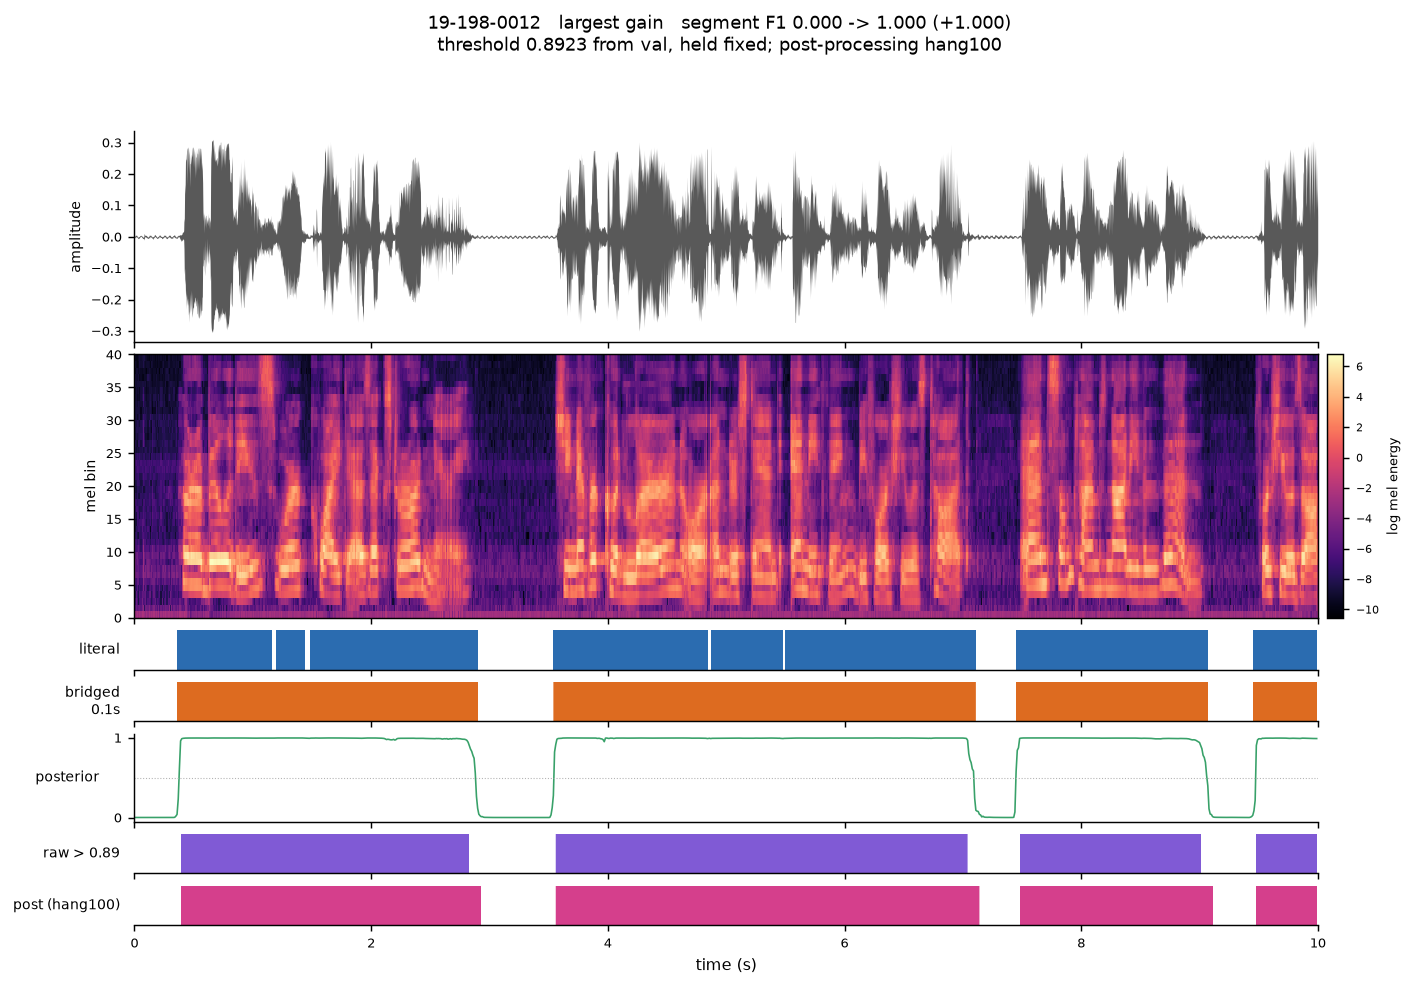
\includegraphics[width=1\linewidth]{postproc_19-198-0012.png}
    \caption{\textbf{Post-processing on a representative clip.} The raw posterior (green) is clean, but the raw decisions (purple) end just inside each speech block because the fading word-tail drops below threshold. Hangover (pink) extends each segment to where the reference ends. Because segment matching with a boundary collar is all-or-nothing, recovering the boundary flips whole segments from miss to match. The hangover length that works, 100 ms, is the same timescale as the gap structure that set the bridging threshold in Sec~\ref{sec: data}: one piece of data analysis informed two decisions.}
    \label{fig:postproc}
\end{figure}

One caveat. Segment F1 with a fixed collar is sensitive to boundary placement and swings sharply on near-perfect clips. The frame-level false-rejection improvement, which has no such cliff, is the more robust corroboration.

\section{Data augmentation}
\label{sec:aug}

Sec~\ref{sec: data} established that the corpus is clean, close-talk, read speech, and the live demo (Sec~\ref{sec:live}) showed what that costs: the clean-trained streaming model tracks speech well but false-fires on finger snaps and table taps. Acoustic augmentation is the fix. It is also the mechanism that builds the held-out test conditions of Sec~\ref{sec:robust}, so it is the single component this report leans on hardest, and it is described here in full: where the acoustics come from, what is applied during training, what is applied to build the test conditions, and what the separation between the two does and does not prove.

Two invariants govern everything below. \emph{Labels are never touched.} Every operation is defined so that speech onsets and offsets stay where the aligner put them, and a test asserts bit-equality of the literal labels, the bridged labels and the segment list before and after augmentation. \emph{Augmentation is a waveform operation.} It is applied before the committed 80\,Hz high-pass and before the log-mel front-end, so the model sees an augmented \emph{recording}, not an augmented feature map. There is no SpecAugment, no time or frequency masking and no speed perturbation anywhere in this work: every operation used has a physical interpretation, which is what makes each of them testable against the label timeline.

\subsection{Where the acoustics come from}

The impulse responses are simulated, not measured, and they are not new to this project. They come from a room-simulation bank I built for a separate keyword-spotting augmentation kit and reused here unchanged. The provenance is worth stating plainly, because that bank was designed for a smart-speaker wake-word problem: two of its design decisions transfer to VAD very well, and one does not transfer at all.

The bank is generated with the image-source method (\texttt{pyroomacoustics}), one shoebox room at a time, with wall absorption derived from a requested RT60 through Sabine's formula and an image-source order cap of 30. The cap is not cosmetic. At the more common cap of 17 the image expansion is truncated long before the decay finishes and the realised RT60 comes out biased low by roughly a quarter: a 3.5\,m room asked for 0.53\,s returns a 0.19\,s response. At order 30 the mean error falls under 10\%. What remains after that is Sabine's own approximation error, which no order cap removes: the median error against the request is 8.2\% and 87.5\% of rooms land within 20\%. Because the realised value is the one that describes the audio, the bank stores it per room, and every RT60 quoted in this report is the realised value rather than the request.

Each rendered path also carries a \texttt{direct\_path\_sample}: the index at which the direct arrival lands. \texttt{pyroomacoustics} renders every image source with an 81-tap fractional-delay sinc centred on the arrival, so the direct sound occupies a window rather than a single sample. The augmenter normalises the impulse response over $\pm 40$ samples around that index and realigns on it. Both numbers come from the renderer rather than from a peak search, which is why a realigned probe lands \emph{exactly} on its original sample index rather than within a sample or two of it.

The one category that does not transfer is the near-field loudspeaker path, and it is refused by construction. It models the device's own driver at 5 to 25\,cm from the microphone, median DRR $+14.3$\,dB and a genuinely near-field path, and exists so a wake-word system can be trained against acoustic echo. Whether a person is speaking has nothing to do with the device's own playback, so \texttt{RIRBank} raises if that category is requested. Only the talker and interferer paths are ever loaded here.

\subsection{One room per clip: why the interferer and the talker share a scene}
\label{sec:aug:scene}

The bank's central design decision, and the one that makes it usable for VAD at all, is that a \emph{scene} is a room rather than a path. Each scene fixes room dimensions, wall material and RT60 once, then places sources inside it: the talker, the interferer and the device loudspeaker. Their impulse responses are rendered in a single \texttt{compute\_rir()} call on that one geometry and share a \texttt{scene\_id}, so the responses belonging to one clip share room dimensions, RT60 and materials instead of being drawn independently. A clip is placed in a room; it is not assembled from unrelated ones. An earlier version of the kit did sample the categories independently, so one clip could put its talker in an 8\,m room and its interferer in a 3\,m one. Nothing physical produces that, and it matters here for a reason specific to what a VAD is being asked to learn.

The discriminative question is whether energy at the microphone came from a vocal tract, and a neural model is free to answer it with any correlate that happens to work on the training set. If the target speech were always reverberant and the interferer always dry, or, more subtly, if the two consistently carried different reverberation times, then ``which decay signature does this component have'' becomes a shortcut that separates the classes perfectly in training and does nothing in a real room, where one set of walls reflects the talker and the television alike. Tying both paths to one room removes that correlate by construction: the interferer's RT60 \emph{is} the talker's RT60, and the only thing left to tell them apart is what they are.

What the shared room preserves is the cue that should carry the decision, which is spatial rather than environmental. Within a scene, the talker and the interferer differ in exactly the ways two real sources in one room differ, namely distance, bearing and height, and Fig~\ref{fig:scenecontrast} shows all three separations. The talker is the nearer source (median 1.27\,m against 1.66\,m). The talker faces the device and the interferer does not: 52\% of talkers fall within $\pm 45^\circ$ of the device front against 22\% of interferers, which is what an unweighted circle gives. And the consequence in the impulse response is a direct-to-reverberant difference: 72\% of talker paths sit below 0\,dB against 88\% of interferer paths, at medians of $-3.3$ and $-4.5$\,dB. Because both sources sit inside the same walls, that DRR gap is a geometry difference and nothing else. Sampled from two unrelated rooms it would be a mixture of geometry and room volume, and the augmentation would be teaching the model a confound.

The azimuth asymmetry in Fig~\ref{fig:scenecontrast}b is deliberate, not an accident of sampling. The talker's bearing is front-weighted (a wrapped normal with $\sigma = 60^\circ$, mixed with a uniform floor drawn 15\% of the time) while the interferer's is uniform over the full circle. A person walks up to a device and talks to it; a television or a dishwasher is placed by the furniture, not by where the user stands. Giving the interferer the talker's front bias would put it where the target is and quietly erase the only spatial contrast the bank has. The uniform floor keeps rear talkers rare rather than absent, which matters because a model that has never heard an off-axis talker fails outright on one. A second constraint keeps the scene physical: talker and interferer are at least 0.5\,m from each other and from the microphone, enforced by rejection inside the scene, so the pair is never co-located, since two point sources at one coordinate is a degenerate impulse-response pair rather than a room, and the far-field condition the reverberation claims to model actually holds. The worst realised separation in the built bank is 0.502\,m, so the constraint binds rather than decorates.

\paragraph{A limitation I found in the room simulation.}
While reviewing the augmentation pipeline, We noticed that we were not actually using the room pairing provided by the bank. The bank associates the talker and interferer responses from the same simulated room, but \texttt{Augmenter} samples the two impulse responses independently from their respective category banks. As a consequence, the talker and interferer in one training example can effectively be placed in two different rooms. We consider this a weakness of the current implementation, since in a real acoustic scene both sources should share the same room characteristics as explained above. The numbers make the difference clear: for correctly paired scenes, the median RT60 difference between talker and interferer is only 0.019,s, whereas independent sampling increases it to 0.181,s, with differences reaching 0.79,s. The corresponding room-volume mismatch has a median factor of 1.47. In a future iteration, We would preserve the bank pairing and sample both responses from the same scene.

What that damages, and what it does not, is worth separating. It does not reintroduce the shortcut, because both categories are drawn from the same marginal room distribution and the reverb and in-room-interferer coins are flipped independently (Sec~\ref{sec:aug:train}): across the training set all four combinations of dry or reverberant speech with dry or reverberant interference occur, and neither RT60 marginal carries information about the label. What is lost is the \emph{within-clip} correlation. Individual mixtures are less physical than the bank allows, and the talker-to-interferer DRR contrast carries a room-mismatch term that no real recording would have. The fix is a one-line change, drawing one \texttt{scene\_id} per clip and indexing both banks with it exactly as the kit's own pipeline does, and it is listed in Sec~\ref{sec:limits} as a fidelity improvement whose effect on the reported numbers is untested, not as a defect that invalidates them.

\subsection{The room bank: dimensions, reverberation time and geometry}

The bank holds 600 scenes, 300 for training and 300 held out to build the test conditions. Table~\ref{tab:rirbank} gives the ranges and Fig~\ref{fig:rirbank} the distributions. Every quantity in both is measured from the rendered impulse response, never read back from the range that was requested.

\begin{table}[H]
    \centering
    \caption{\textbf{The simulated room bank}, measured from the built bank rather than from the requested ranges. Each split holds 300 scenes, and each scene contributes one talker path and one interferer path, so a split supplies 300 impulse responses per category. The two splits are drawn from identical ranges under different seeds and share no room, no source position and no impulse response. DRR is the direct-to-reverberant ratio at the microphone.}
    \label{tab:rirbank}
    \small
    \begin{tabular}{lrr}
        \toprule
        Quantity & Train split & Held-out (\emph{hard}) split \\
        \midrule
        Scenes (rooms) & 300 & 300 \\
        Room length (m) & 3.01--7.98 & 3.03--7.99 \\
        Room width (m) & 3.01--8.00 & 3.01--7.99 \\
        Ceiling height (m) & 2.40--3.20 & 2.40--3.20 \\
        Volume (m$^3$), median (range) & 77 (25--183) & 77 (27--169) \\
        RT60 requested (s) & 0.20--0.90 & 0.20--0.90 \\
        RT60 realised (s), median (range) & 0.53 (0.16--1.04) & 0.52 (0.17--0.97) \\
        \midrule
        Talker distance (m), median (range) & 1.33 (0.50--4.69) & 1.22 (0.50--4.73) \\
        Talker height (m) & 1.01--1.80 & 1.01--1.80 \\
        Talker DRR (dB), median (range) & $-3.6$ ($-14.8$ to $+9.6$) & $-3.2$ ($-13.6$ to $+9.9$) \\
        Interferer distance (m), median (range) & 1.69 (1.00--5.94) & 1.63 (1.00--5.66) \\
        Interferer height (m) & 0.30--2.00 & 0.31--1.99 \\
        Interferer DRR (dB), median (range) & $-4.5$ ($-13.7$ to $+8.4$) & $-4.5$ ($-13.0$ to $+5.2$) \\
        Talker--interferer separation (m) & 0.50--3.43 & 0.50--3.43 \\
        \bottomrule
    \end{tabular}
\end{table}

\begin{figure}[H]
    \centering
    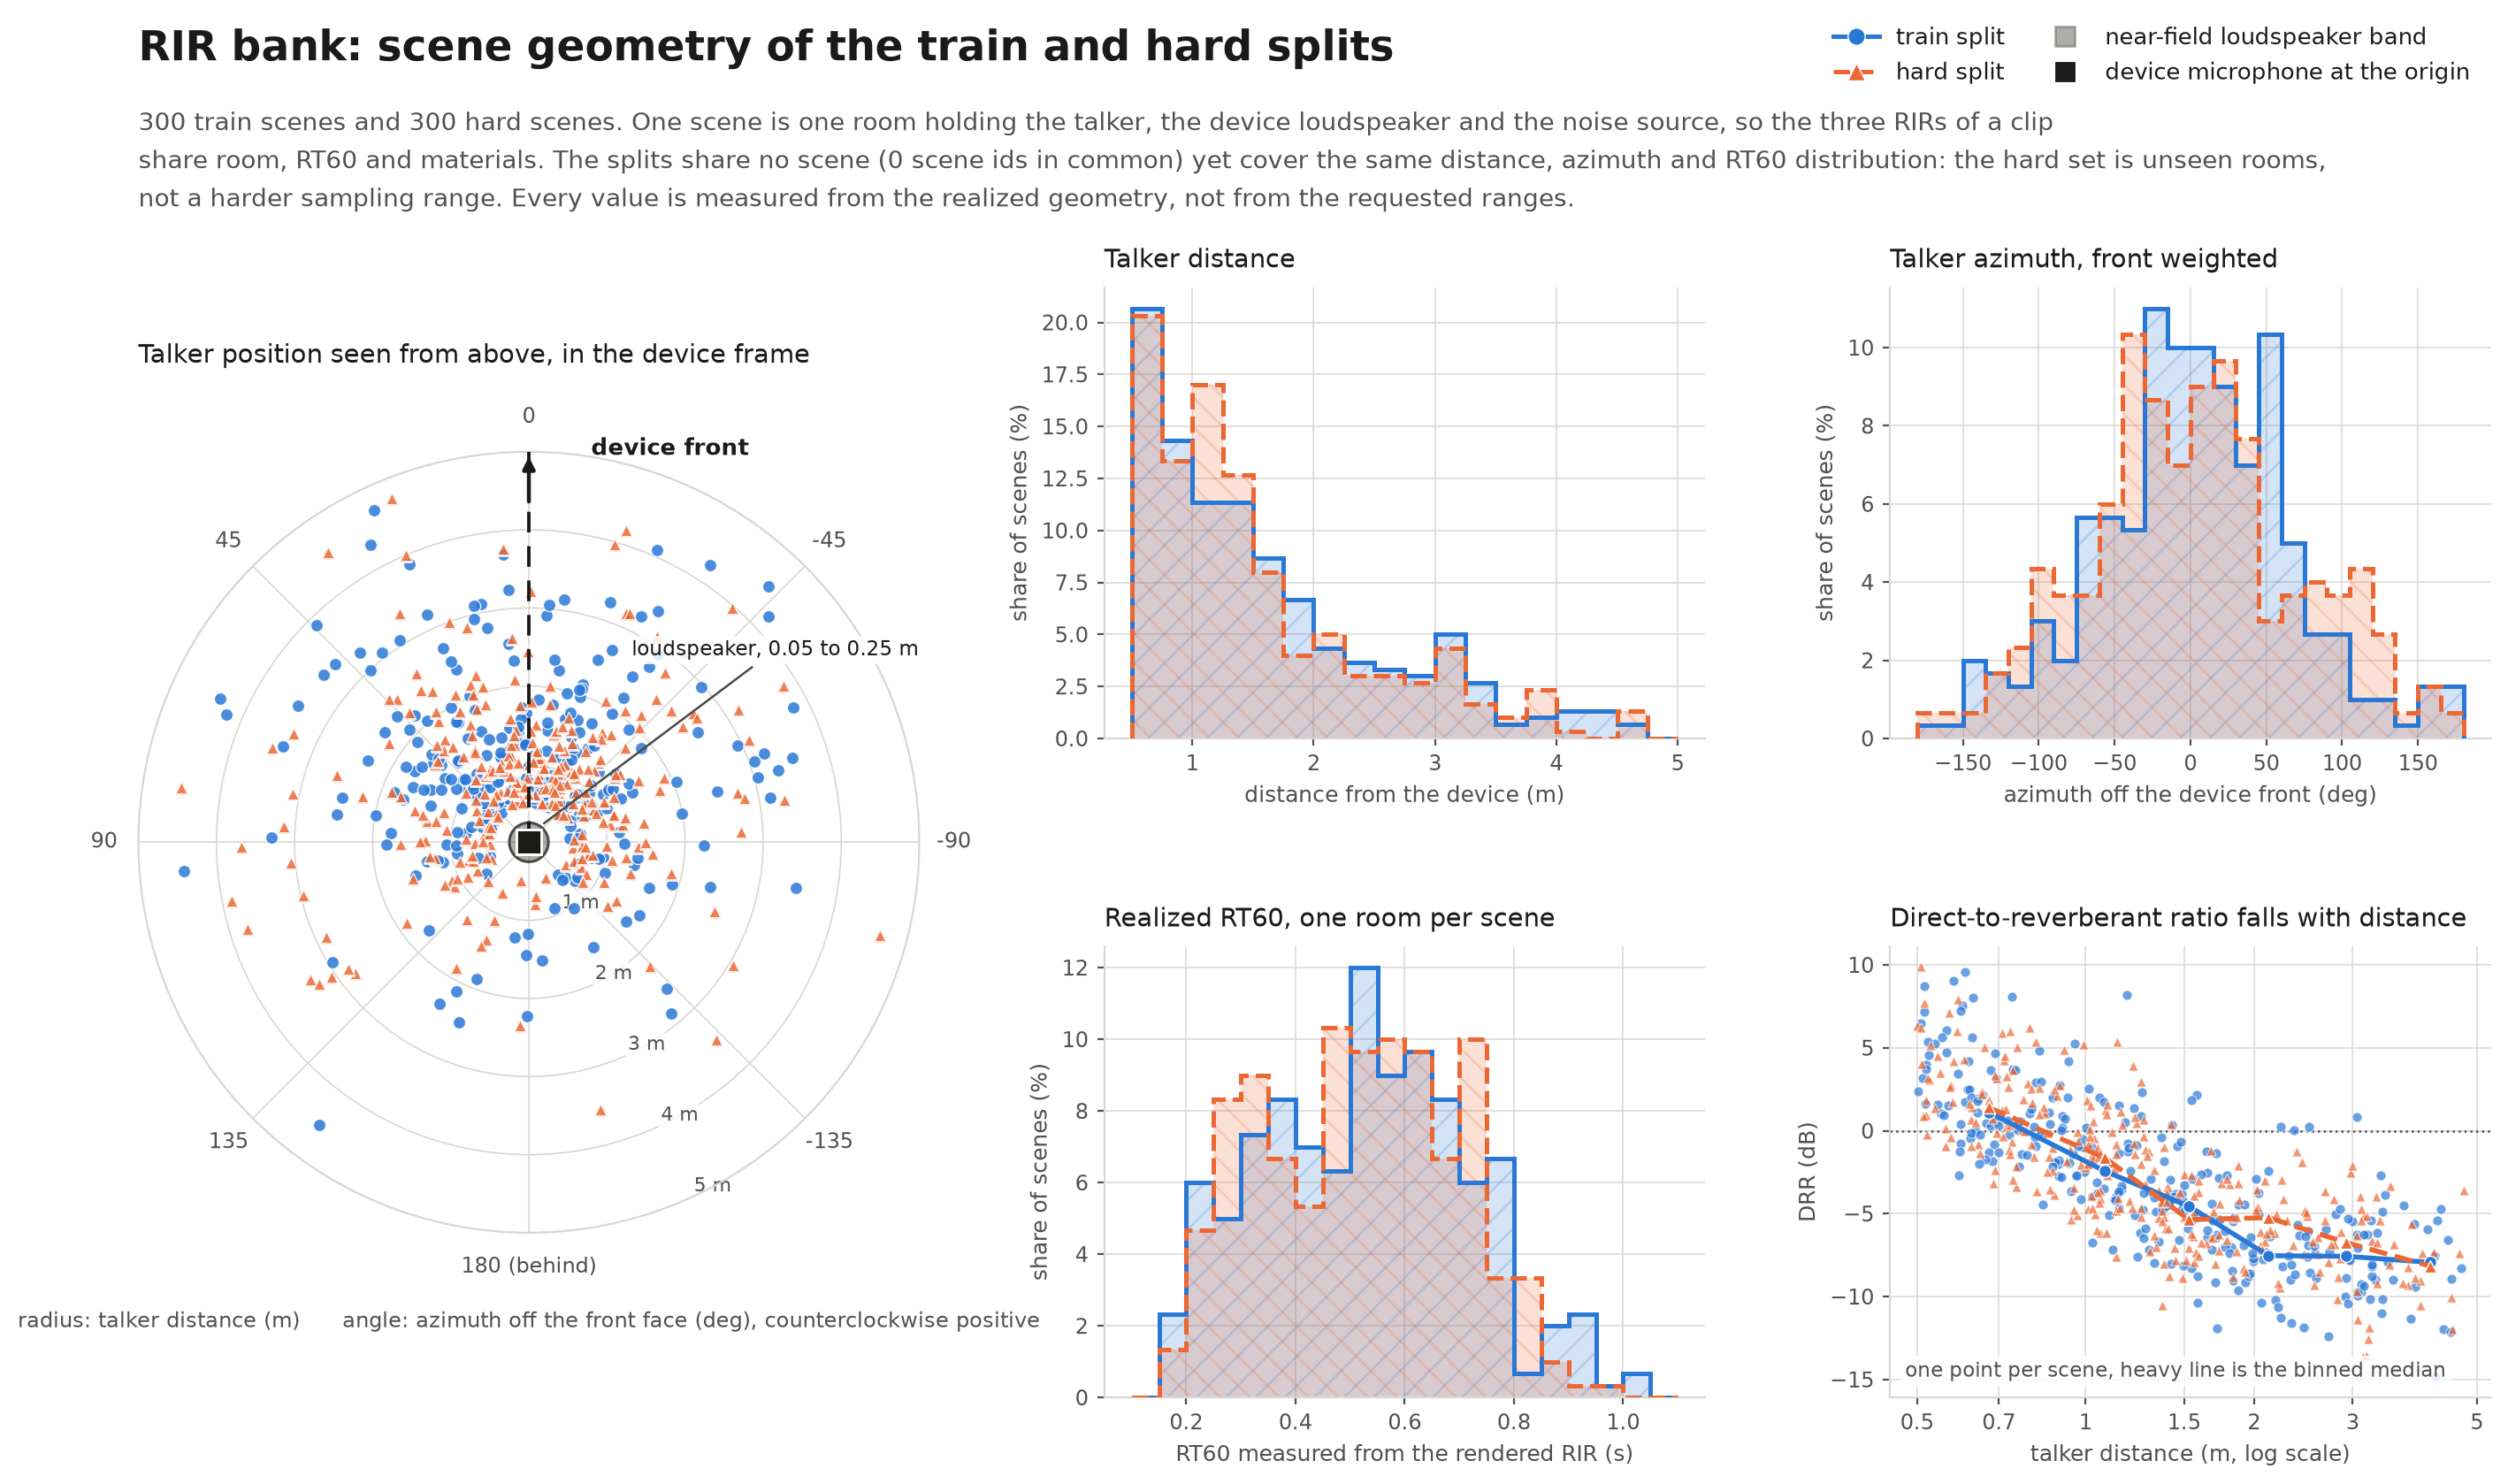
\includegraphics[width=1\linewidth]{rir_distribution.png}
    \caption{\textbf{The room bank: scene geometry of the train and hard splits.} One point is one scene, that is one room holding the talker, the device loudspeaker and the noise source, so the three impulse responses of a clip are physically coherent. Left: talker position in the device frame, radius in metres, angle off the front face. The splits share no scene identifier, yet the distance, azimuth and RT60 histograms overlap closely, so the hard split is unseen rooms rather than a harder sampling range. Right: the direct-to-reverberant ratio falls with distance and is below 0 dB for 72\% of scenes, which is why reverberation is applied with the speech-active level restored afterwards. Every value is measured from the rendered impulse response, not from the requested ranges.}
    \label{fig:rirbank}
\end{figure}

\begin{figure}[H]
    \centering
    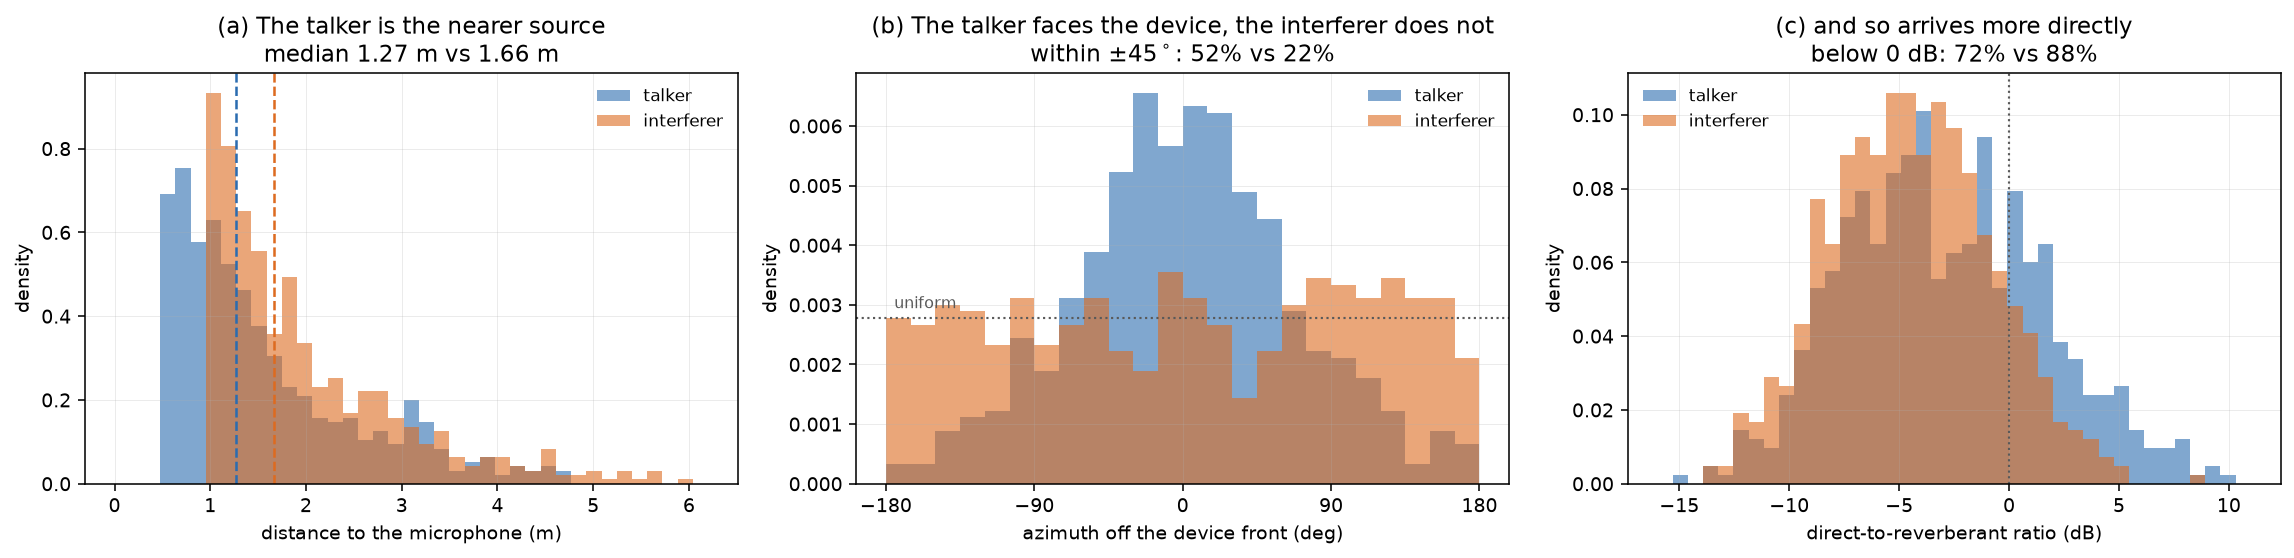
\includegraphics[width=1\linewidth]{rir_scene_contrast.png}
    \caption{\textbf{Talker against interferer inside the same room}, both splits pooled, since the contrast is within a scene and does not depend on the split. Fig~\ref{fig:rirbank} shows that the two \emph{splits} match; this shows how the two \emph{sources} of one scene differ. (a) The talker is the nearer source. (b) The talker's bearing is front-weighted while the interferer's is uniform, because a user walks up to a device and a television is placed by the furniture. (c) The interferer is therefore the more reverberant-dominated of the two. All three separations are geometry inside one room, which is exactly what makes them a usable contrast: had the two sources been drawn from unrelated rooms, the same gaps would have confounded geometry with room size.}
    \label{fig:scenecontrast}
\end{figure}

Rooms are shoeboxes between 3.0 and 8.0\,m on each horizontal side with ceilings from 2.40 to 3.20\,m, giving volumes from 25 to 183\,m$^3$ around a median of 77\,m$^3$. That is the domestic and small-office range: living rooms, kitchens, bedrooms, meeting rooms. It is deliberately not a concert hall, a corridor, a stairwell or a car cabin, and the robustness claim of Sec~\ref{sec:robust} should be read as scoped to that envelope.

Reverberation time is requested uniformly over 0.20 to 0.90\,s and realised over 0.16 to 1.04\,s in training and 0.17 to 0.97\,s held out, medians 0.53\,s against 0.52\,s. Both ends of that range are meaningful for this task, and the reason is the frame grid. Near 0.2\,s the tail barely outlives a handful of 10\,ms frames and reverberation is close to a colouration. Near 0.9\,s the tail runs across roughly 90 frames, far longer than the 100\,ms gap threshold that Sec~\ref{sec: data} used to define the bridged labelling convention, so energy from a word is still decaying well past the point where the reference calls the speech over. That is exactly the mechanism behind the failure this report set out to fix: a clean-trained VAD reads a decaying tail as continuing speech and over-extends its offsets. Training across the full 0.2 to 0.9\,s range is what teaches it that a tail is not a voice, and it is why reverberation is treated as a first-class augmentation here rather than as a minor addition to noise.

The two splits are generated from identical ranges under different seeds (20240101 and 987654321). They share no scene, yet their distance, azimuth and RT60 distributions overlap closely (Fig~\ref{fig:rirbank}): median talker distance 1.33\,m against 1.22\,m, median realised RT60 0.53\,s against 0.52\,s, and 52\% of talkers within $\pm 45^\circ$ of the device front in both. That overlap is the point. The held-out set is \emph{unseen rooms}, not a harder sampling range, which is what makes the reverberant columns of Table~\ref{tab:robust} a generalisation result rather than an extrapolation into conditions the sampler never offered during training.

The talker distance distribution is skewed towards the near field (median 1.33\,m against a uniform-request midpoint of 2.75\,m) and this is expected: a 4\,m room cannot hold a talker 5\,m from the device, so the far half of the requested range is truncated far more often than the near half. The bank draws the azimuth first and then clips the distance range to what that bearing can physically reach, rather than drawing a distance and rejecting out-of-room points, since a rejection scheme would delete exactly the bearings pointing at a near wall and leave a hole in the angular coverage. All twelve $30^\circ$ bearing bins are occupied in both splits for both source types. Trading a truthful distance histogram for a false azimuth one would have been the worse bug.

\subsection{Training-time augmentation}
\label{sec:aug:train}

Table~\ref{tab:augsettings} gives the settings. The order of operations is fixed and is physical: reverberate the talker, then add the interferer at the microphone. Reversing it would be a real error rather than a stylistic one, because interference added before the convolution would be filtered by the \emph{talker's} impulse response and would acquire the target's distance, bearing and propagation delay instead of its own.

\begin{table}[H]
    \centering
    \caption{Training-time augmentation settings and the four fixed test conditions. Training draws rooms from the \emph{train} split and recordings from the MUSAN training pool; every test condition draws rooms from the held-out \emph{hard} split and recordings from the MUSAN test pool. $p(\text{room on interferer})$ is the probability that the additive interferer is itself convolved with an interferer-path impulse response.}
    \label{tab:augsettings}
    \small
    \begin{tabular}{lcccc}
        \toprule
        & $p(\text{reverb})$ & $p(\text{interferer})$ & $p(\text{room on interferer})$ & SNR (dB) \\
        \midrule
        Training            & 0.5 & 0.8 & 0.5 & $\mathcal{U}(0, 20)$ \\
        Validation          & \multicolumn{4}{c}{none; validation stays clean, for selection and thresholding} \\
        \midrule
        Test: clean         & 0 & 0 & --- & --- \\
        Test: noise         & 0 & 1 & 0 & $\mathcal{U}(0, 10)$ \\
        Test: reverb        & 1 & 0 & --- & --- \\
        Test: noise+reverb  & 1 & 1 & 1 & $\mathcal{U}(0, 10)$ \\
        \bottomrule
    \end{tabular}
\end{table}

\paragraph{Reverberation, on half the clips.} Speech is convolved with a talker-path impulse response and then realigned. \texttt{np.convolve} places the direct arrival of input sample 0 at output index \texttt{direct\_path\_sample}, so the augmenter slices from that index and input sample $t$ lines up with output sample $t$ again. Without that slice the whole utterance would slide later by the time of flight, 14\,ms at 4.7\,m and more than one frame, and every label would be stale by that amount. Both halves of this are tested: a probe impulse convolved with a sample of the bank's rooms comes back with its peak at exactly the original index, and on speech the measured energy onset moves by at most one frame.

Level is handled separately from alignment, and the reason is quantitative. Normalising the impulse response by its direct-path energy keeps the direct sound at the level it left at, which is what makes the convolution physically meaningful, but it does not keep the \emph{total} level fixed, and in this bank it is nowhere near fixed, because 72\% of talker paths have a DRR below 0\,dB, meaning that in most of these rooms the reverberant field carries more energy than the direct sound. The measured overall gain runs from $+0.7$ to $+17.5$\,dB across rooms. Left alone that is a second, uncontrolled variable riding on top of the one being tested, and it does not wash out downstream: the features are normalised with fixed training statistics, so a 17\,dB offset reaches the model intact. The augmenter therefore restores the speech-active RMS after convolution. Reverberation then varies the smearing and not the loudness, which is the variable the experiment is about. A test asserts the restored gain is unity to within $10^{-4}$ while the unrestored gain exceeds 1.5 on some rooms.

\paragraph{Additive interference, on 80\% of clips.} A MUSAN music or ambient-noise recording is randomly cropped to the clip length, or tiled if it is shorter, and added at an SNR drawn uniformly from 0 to 20\,dB. Two details are load-bearing.

First, the SNR is measured over speech-active frames only, for the speech and for the interferer alike. Measuring speech power over the whole clip would fold the silences into it and make the realised SNR depend on how talkative the clip happens to be. This corpus is 80.7\% speech overall, but individual clips range from 49\% to 93\%, so the whole-clip choice would move the true SNR by several dB from clip to clip and the SNR axis of the whole experiment would stop meaning anything. Measuring the interferer over the same frames closes the other half of the same hole, since a recording is rarely stationary across a clip.

Second, the interferer is placed in a room only half the time. Always convolving would be wrong: MUSAN recordings already carry the acoustics of wherever they were captured, and a second convolution double-reverberates them. Never convolving would be wrong in the other direction, leaving every interferer anechoic against a talker that is in a room half the time, which is the shortcut of Sec~\ref{sec:aug:scene} reintroduced by the back door. Half and half spans both cases and leaves neither marginal informative about the label.

\paragraph{Randomness and reproducibility.} Each item draws from \texttt{default\_rng([seed, epoch, index])}, so a clip gets a different room, a different recording and a different SNR every epoch, while a given \texttt{(seed, epoch, index)} reproduces the draw exactly and the result does not depend on how many dataloader workers are running or on batch order. What was actually applied is recorded per clip, the impulse-response ids, the interferer filename and the realised SNR, so any training example can be rebuilt and listened to.

\paragraph{Validation stays clean.} Augmentation is applied to the training partition only. Checkpoint selection and the operating threshold are both chosen on clean validation, for the augmented run and the clean run alike. This is a deliberate choice with a cost on each side. Against it: the augmented model is selected on a distribution it was not trained on, which is not the distribution it will be deployed in. For it: the two runs are then selected against an identical criterion, so the clean-versus-augmented comparison in Table~\ref{tab:robust} is a comparison of models rather than of selection rules, and every threshold reported there is a number frozen on clean data and transferred unchanged to noisy data rather than tuned per condition. For a report whose central claim is that augmentation buys robustness at almost no clean cost, holding the selection rule fixed is the more important property.

\subsection{Test-time augmentation: four fixed, held-out conditions}

The four test conditions are built from the clean test split by the same \texttt{Augmenter} class with different settings (Table~\ref{tab:augsettings}). That reuse is the point: the evaluation conditions are not a second implementation that could quietly drift from the training one. Three properties make them usable as a benchmark.

\emph{They are fixed.} The generator is seeded by \texttt{default\_rng([1234, index])} with no epoch term, so a condition is byte-identical every time it is rebuilt. Every system in Table~\ref{tab:robust} (the BiGRU, the causal model, Silero and WebRTC) is scored on exactly the same audio, so differences between rows are differences between systems and not between draws.

\emph{They are held out.} Rooms come from the \emph{hard} split and recordings from the MUSAN test pool. No room and no recording heard in training appears in any test condition (Sec~\ref{sec:aug:disjoint}).

\emph{They are harder than training, on the axis that matters.} Training draws SNR uniformly from 0 to 20\,dB; the test conditions draw from 0 to 10\,dB, the harder half of the training range. Reverberation is applied with probability 1 rather than 0.5. The conditions are also factorial by design: \texttt{noise} uses a dry interferer and no room on the talker, \texttt{reverb} uses a room and no interferer, and \texttt{noise+reverb} puts talker and interferer both in rooms. The matrix therefore separates additive interference from room acoustics from their combination, instead of collapsing to one aggregate ``noisy'' number.

One asymmetry should be read as deliberate. The \texttt{noise} condition sets $p(\text{room on interferer}) = 0$, so its interferer carries only its own recorded acoustics, while \texttt{noise+reverb} sets it to 1 and training sits between the two at 0.5. The test conditions bracket the training placement rather than reproducing it, which is the more informative arrangement: the two endpoints bound what the middle would give.

\subsection{Disjointness, and its limits}
\label{sec:aug:disjoint}

The separation between training and test resources is enforced in code and asserted by tests, not assumed. On the room side, the two splits are generated from different seeds and their ids are namespaced (training from 0, held out from 500000), so no room, talker position or interferer position is shared, and a test checks that the two id sets are disjoint for every category.

On the recording side, \texttt{musan\_pool} partitions files by the MD5 hash of the path relative to the MUSAN root, taking bucket $< 80$ as training. A hash rather than a shuffle, because the partition must not depend on directory order, on how many files happen to be present, or on any seed: a recording lands in the same pool on every machine and in every run, which is what makes the pools genuinely disjoint rather than disjoint by luck. Of the 1590 files available, 1290 (538 music, 752 noise) go to training and 300 (122 music, 178 noise) to test, with zero overlap and complete coverage, all three properties asserted. A final test constructs the training augmenter and the test augmenter side by side and checks that they share no impulse-response id and no file at all.

\paragraph{What are the limits} Three limits, stated here so Sec~\ref{sec:robust} can be read at its true strength.

First, both room splits come from the same simulator under the same priors on size, absorption and geometry. The experiment measures generalisation to unseen rooms drawn from a known distribution. It does not measure generalisation to measured impulse responses, to non-shoebox geometry, or to rooms outside the 25 to 183\,m$^3$ and 0.2 to 0.9\,s envelope. A bank of real measured responses would be a strictly stronger test and is the obvious next step.

Second, the interferer pool contains only music and ambient noise; the MUSAN speech subset is not used. As a result, the experiments do not include competing speakers or speech babble, which are particularly challenging for VAD because the interferer is itself speech and the desired label depends on which speaker is considered the target. The robustness results in Sec~\ref{sec:robust} should therefore be interpreted specifically as robustness to non-speech interference. A stronger evaluation would also include competing talkers, for example by drawing interferer speech from the labelled dataset. I did not include this additional condition because of time constraints and other project priorities. 

Third, the mixing model is additive at the microphone with no device chain: no Lombard effect on the talker, no automatic gain control, no compression or codec, and a single microphone. Each of those is a genuine distribution shift between this augmentation and a deployed device.

\newpage

\section{Robustness to noise and reverberation}
\label{sec:robust}

Sec~\ref{sec: data} predicted that a model trained on this corpus would never learn to handle noise, and the live demo (Sec~\ref{sec:live}) made the prediction concrete. This section measures the size of that gap and what the augmentation of Sec~\ref{sec:aug} does to it.

The four conditions scored below (clean, noise, reverb, and noise-plus-reverb) are built from the clean test split using held-out rooms and held-out recordings under a fixed seed (Table~\ref{tab:augsettings}), so no room and no recording heard in training appears here, and every system in this section is scored on byte-identical audio.

\subsection{Results: the four models on clean and noisy test}

We trained a second copy of each architecture with augmentation, identical in every other respect, including the 30-epoch budget and early-stopping patience (Table~\ref{tab:cost}), selecting on clean validation. All thresholds in Table~\ref{tab:robust} are the operational threshold, chosen on clean validation to minimise misses while meeting a 100-false-alarms-per-hour budget, then frozen and applied unchanged to every test condition.

\begin{table}[H]
    \centering
    \caption{The four models on clean and noisy test. Best value per column in bold. The two rows marked $\dagger$ are the clean-trained models under unseen noise; their collapsed metrics are set in italics. AUC is ROC-AUC, Rec.\ is recall, Fr.\ F1 is frame F1, and Sg.\ F1 is segment F1.}
    \label{tab:robust}
    \setlength{\tabcolsep}{1.5pt}
    \scriptsize
    \begin{tabular}{lllrrrrrrrr}
        \toprule
        Model & Train. & Test & EER $\downarrow$ & AUC $\uparrow$ & FRR $\downarrow$ & FAR $\downarrow$ & Rec. $\uparrow$ & Fr. F1 $\uparrow$ & FA/h $\downarrow$ & Sg. F1 $\uparrow$ \\
        \midrule
        BiGRU       & no aug.   & clean & \textbf{2.02\%} & \textbf{0.9951} & 2.37\%  & 1.76\%                       & 97.63\%          & \textbf{98.62\%} & 80.5                          & 0.153 \\
        BiGRU       & no aug.   & noise$^{\dagger}$ & \textit{30.85\%} & \textit{0.7492} & 1.71\%  & \textit{65.20\%}             & 98.29\%          & 92.83\%          & \textit{1213.9}               & 0.066 \\
        BiGRU       & augmented & clean & 2.05\%          & 0.9948          & 2.46\%  & 1.77\%                       & 97.54\%          & 98.57\%          & 78.5                          & 0.203 \\
        BiGRU       & augmented & noise & \textbf{3.58\%} & \textbf{0.9902} & 5.20\%  & \textbf{2.32\%}              & 94.80\%          & \textbf{97.09\%} & 110.7                         & \textbf{0.338} \\
        Causal 1 s  & no aug.   & clean & 2.47\%          & 0.9931          & 5.76\%  & 1.20\%                       & 94.24\%          & 96.91\%          & 54.4                          & \textbf{0.409} \\
        Causal 1 s  & no aug.   & noise$^{\dagger}$ & \textit{25.80\%} & \textit{0.8165} & 3.46\%  & \textit{57.29\%}             & 96.54\%          & 92.66\%          & \textit{1326.7}               & 0.095 \\
        Causal 1 s  & augmented & clean & 2.96\%          & 0.9930          & 6.60\%  & 1.25\%                       & 93.40\%          & 96.46\%          & \textbf{48.3}                 & 0.350 \\
        Causal 1 s  & augmented & noise & 6.89\%          & 0.9786          & 12.39\% & 3.59\%                       & 87.61\%          & 93.03\%          & 159.0                         & 0.185 \\
        \bottomrule
    \end{tabular}
\end{table}

Operational thresholds: BiGRU 0.6287 (no aug.) and 0.5491 (aug.); causal 0.7548 and 0.8021. Precision is above 99\% for every row and is omitted for space.

\paragraph{What augmentation does.} The result is very clear and holds across both architectures. For the BiGRU, augmentation changes clean EER only from 2.02\% to 2.05\%, but on noise from 30.85\% to 3.58\%, and noisy false alarms fall from 1214 to 111 per hour. For the causal model, clean EER moves from 2.47\% to 2.96\%, while noisy EER improves from 25.80\% to 6.89\% and false alarms drop from 1327 to 159 per hour. Augmentation has almost no clean-performance cost and a very large robustness benefit.

\paragraph{The clean model's failure mode is false alarms.} Under noise the clean-trained models' false-accept rate exceeds 57\%, while their miss rate actually drops (BiGRU 2.37\% to 1.71\%). They stop discriminating and call almost everything speech. This is the numerical form of the finger-snap and table-tap failure in the demo: the model fires on non-speech transients it never learned to reject. The augmented models' false-accept rate under noise is 2 to 4\%.

\begin{figure}[H]
    \centering
    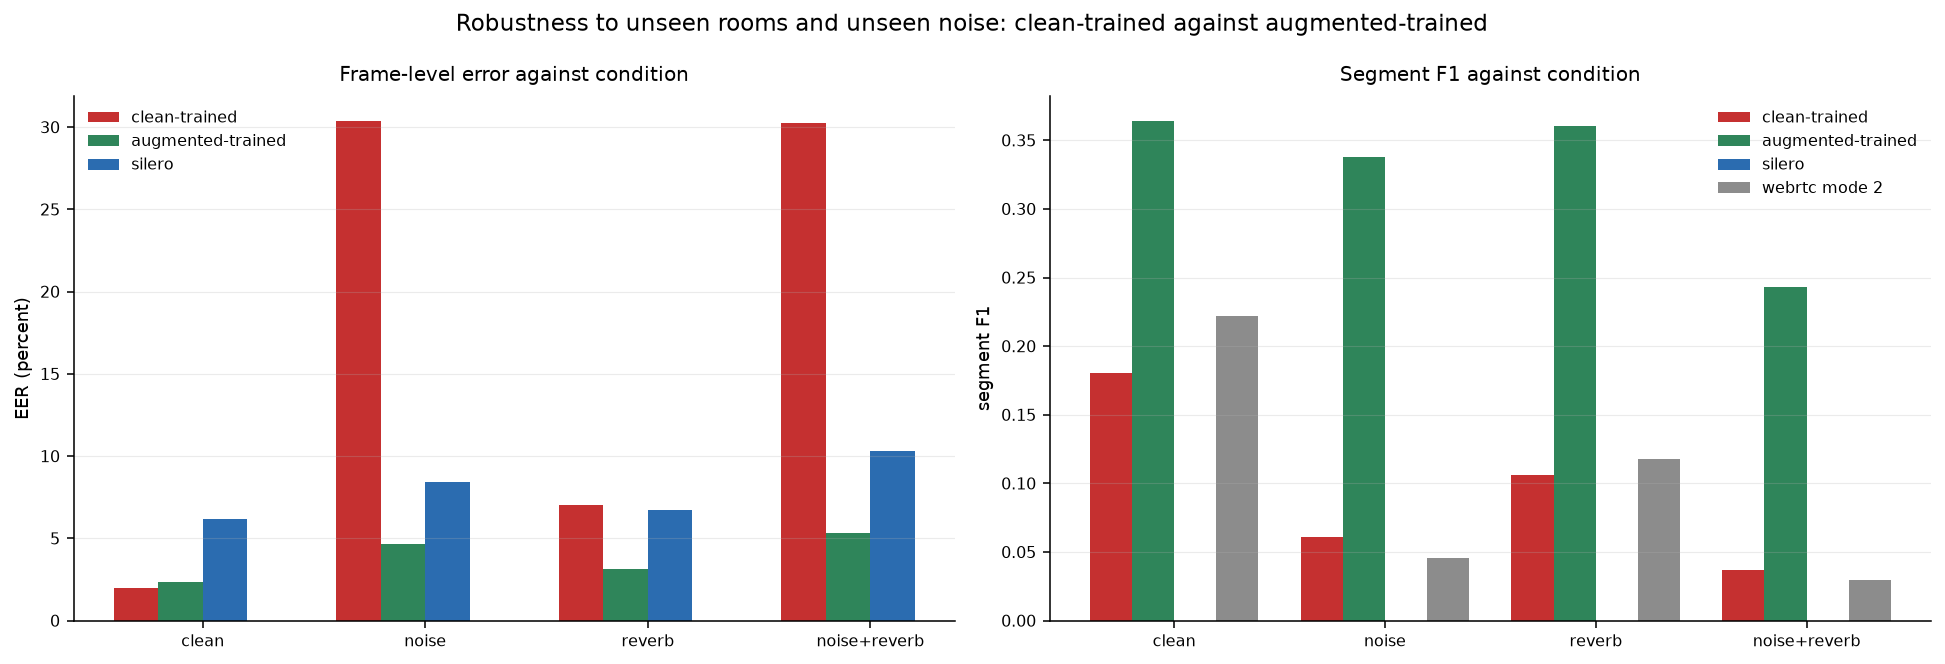
\includegraphics[width=1\linewidth]{robustness_matrix.png}
    \caption{\textbf{Robustness of the offline model to unseen rooms and unseen noise, across four conditions.} Left: EER by condition. The clean-trained model (red) collapses under noise; the augmented model (green) holds within a few points of its clean number across every condition and, on noise-plus-reverb, beats Silero (blue). Centre and right: segment F1 at the operational threshold and at each system's best clean-validation threshold. The WebRTC bars in this figure are mode 2; the validation-selected mode is mode 3 (Sec~\ref{sec:clean}), so the WebRTC bars here are indicative only.}
    \label{fig:robustbigru}
\end{figure}

\begin{figure}[H]
    \centering
    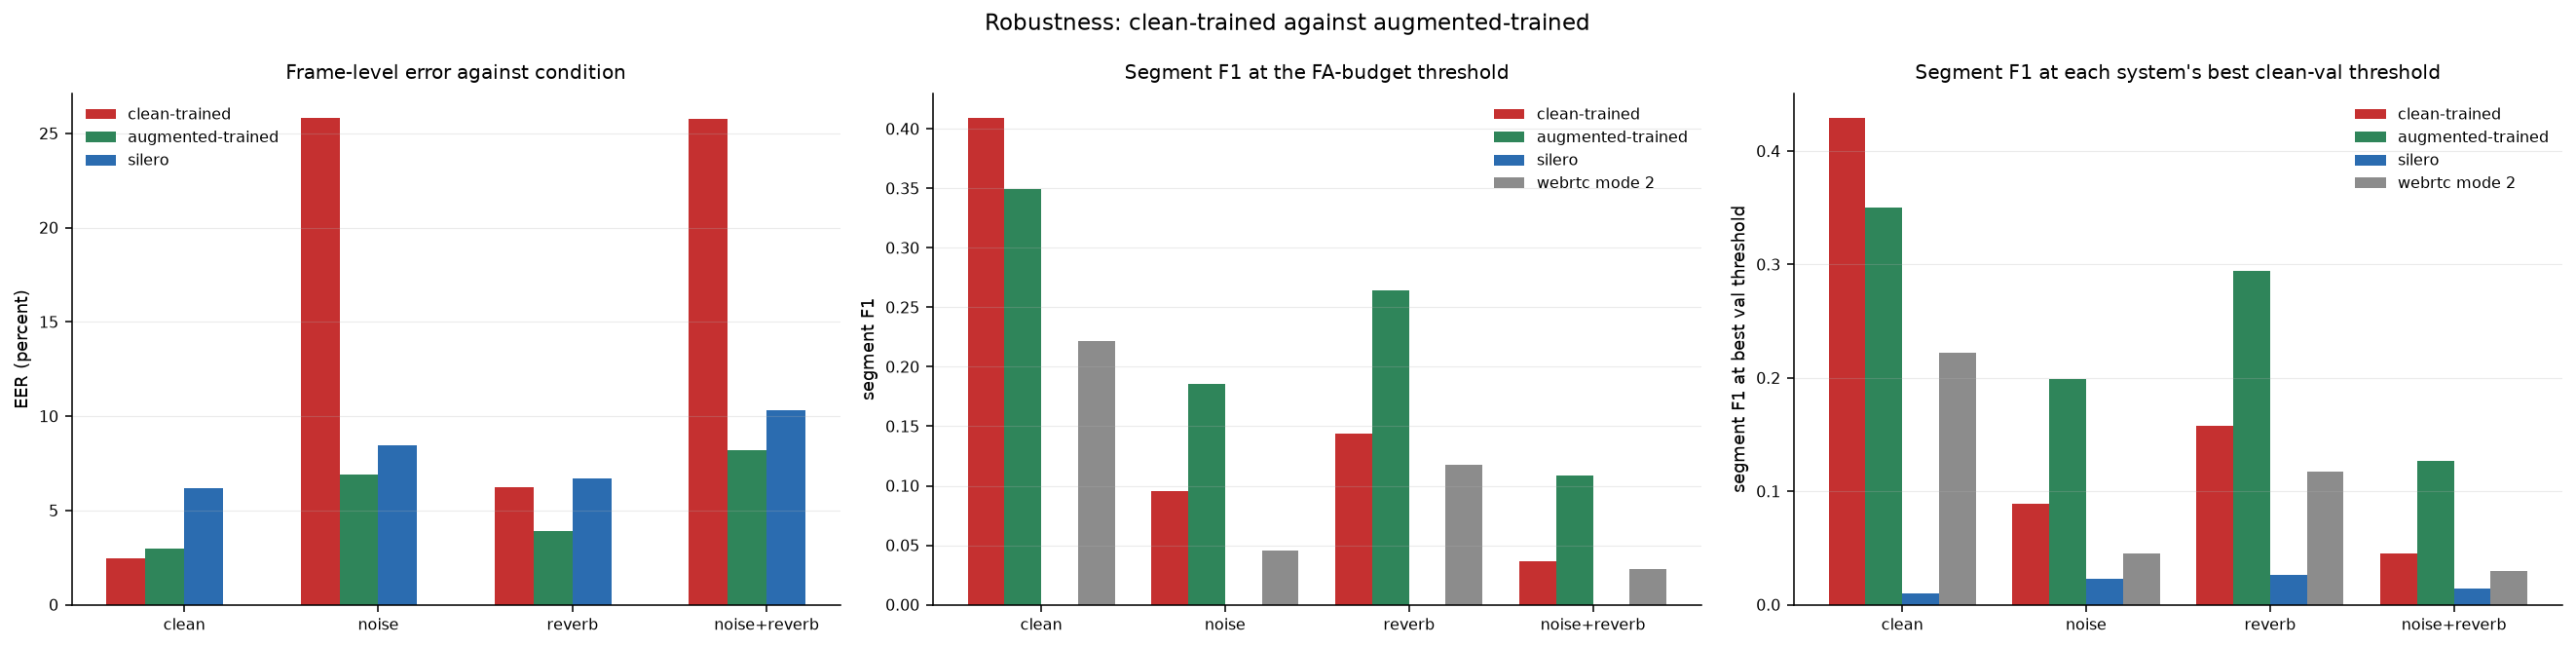
\includegraphics[width=1\linewidth]{robustness_causal.png}
    \caption{\textbf{Robustness of the streaming model.} The same pattern: augmentation makes the causal model robust (green versus red), but streaming-plus-noise is the hardest combination. WebRTC bars are mode 2, as above.}
    \label{fig:robustcausal}
\end{figure}

\subsection{BiGRU against causal attention: a genuine trade-off}

For the two augmented models, which are the realistic deployment candidates, the comparison is not one-sided. Table~\ref{tab:tradeoff} isolates it.

\begin{table}[t]
    \centering
    \caption{The two augmented models on clean and noisy test, at their operational thresholds. Better of the two architectures within each condition in bold.}
    \label{tab:tradeoff}
    \setlength{\tabcolsep}{4pt}
    \small
    \begin{tabular}{lrrrr}
        \toprule
        Augmented models & Clean BiGRU & Clean causal & Noise BiGRU & Noise causal \\
        \midrule
        EER $\downarrow$        & \textbf{2.05\%}  & 2.96\%           & \textbf{3.58\%}  & 6.89\% \\
        ROC-AUC $\uparrow$      & \textbf{0.9948}  & 0.9930           & \textbf{0.9902}  & 0.9786 \\
        Recall $\uparrow$       & \textbf{97.54\%} & 93.40\%          & \textbf{94.80\%} & 87.61\% \\
        Frame F1 $\uparrow$     & \textbf{98.57\%} & 96.46\%          & \textbf{97.09\%} & 93.03\% \\
        FA/hour $\downarrow$    & 78.5             & \textbf{48.3}    & \textbf{110.7}   & 159.0 \\
        Segment F1 $\uparrow$   & 0.203            & \textbf{0.350}   & \textbf{0.338}   & 0.185 \\
        \bottomrule 
    \end{tabular}
\end{table}

The BiGRU is clearly the stronger frame-level classifier and the more robust model under noise. But the causal model has fewer false alarms on clean audio (48 versus 78 per hour) and substantially higher clean segment F1 (0.350 versus 0.203) at the operational threshold. So the offline model is not simply better: the streaming model is cleaner on clean segments, while the offline model degrades less under noise. The honest headline is that streaming-plus-noise is the hardest regime. The augmented causal model sits at 6.89\% under noise against the augmented BiGRU's 3.58\%, a robustness cost to streaming beyond the clean-condition cost. For deployment in variable acoustic conditions the augmented BiGRU is the strongest overall choice.

\paragraph{Against Silero.} At its own validation-selected operational threshold, Silero reaches 6.18\% EER on clean test with 75.5\% recall and a frame F1 of 85.9\%. Under noise its recall falls to 36.4\% and its frame F1 to 53.3\%. The augmented BiGRU under the same noise keeps 94.8\% recall and 97.1\% frame F1. The learned models, especially the augmented BiGRU, outperform Silero substantially in both discrimination and recall at the chosen operating regime.

\paragraph{The result.} Across both architectures, augmentation with unseen rooms and unseen noise transforms robustness (30.85\% to 3.58\% EER for the offline model) at essentially no cost on clean audio. This is a domain-trained model made robust with simulated acoustics, evaluated fairly on held-out conditions, not a claim of universal superiority.

\section{Operating thresholds: two families, two objectives}
\label{sec:thresholds}

All thresholds are chosen on clean validation and frozen, but there are two families serving different objectives, and they should not be mixed in one column without labelling. Table~\ref{tab:thresholds} lists both.

\begin{table}[t]
    \centering
    \caption{The two threshold families, both chosen on clean validation and frozen. The primary deployment threshold is in bold.}
    \label{tab:thresholds}
    \small
    \begin{tabular}{lcc}
        \toprule
        System & \shortstack{Operational threshold\\ \scriptsize min.\ misses at 100 FA/h} & \shortstack{Segment-F1 threshold\\ \scriptsize max.\ segment F1} \\
        \midrule
        BiGRU, no augmentation      & 0.6287          & 0.9152 \\
        BiGRU, augmented            & \textbf{0.5491} & 0.8871 \\
        Causal 1 s, no augmentation & 0.7548          & 0.7970 \\
        Causal 1 s, augmented       & 0.8021          & 0.7252 \\
        Silero                      & 0.9997          & 0.7066 \\
        \bottomrule
    \end{tabular}
\end{table}

The main results table uses the operational family, because minimising misses under a false-alarm budget is the deployment criterion. The segment-F1 family is reported as a secondary analysis, and it teaches something useful. For the augmented BiGRU, moving from the operational threshold 0.5491 to the segment-optimised 0.8871 raises clean segment F1 from 0.203 to 0.479 and cuts clean false alarms from 78.5 to 26.2 per hour, but recall drops from 97.5\% to 93.8\%. More importantly, on noisy data that same frozen threshold gives only 87.2\% recall, and noisy segment F1 actually falls from 0.338 to 0.270. The segment-optimised threshold is excellent for clean boundaries, but the operational threshold generalises better to noise. This is why 0.5491 is the primary deployment threshold for the augmented BiGRU: if robustness in the field matters, the operating point that meets the false-alarm budget is the one to ship.

\section{Live streaming demo}
\label{sec:live}

The streaming model runs live on microphone input. This is the same model, unmodified, that produces the offline numbers. Audio is captured, resampled to 16 kHz, passed through the identical front-end (the 80 Hz high-pass and log-mel features, normalised with the saved training statistics rather than statistics recomputed on the live audio), and fed frame-by-frame through the bounded-window streaming path. A scrolling display shows the log-mel, the speech probability, and the thresholded decision in three aligned panels.

\paragraph{Faithfulness.} Replaying a file through the live path and comparing against the offline forward pass, the per-frame decisions agree on 1402 of 1402 frames, with a maximum probability difference of $9\times10^{-5}$. The live path is not an approximation: batch evaluation and live streaming compute the same thing, which is what makes the offline numbers a valid statement about live behaviour. This was the single most likely failure mode, a live front-end that silently mismatches training, and it did not occur.

\paragraph{Latency and memory.} End-to-end latency is 245 ms, fully itemised: a
30 ms audio block, a 100 ms margin so the zero-phase high-pass reproduces the
offline filter exactly, a 15 ms analysis-window tail, and 100 ms of model
lookahead. Every term is algorithmic; none of it is compute time. The zero-phase
high-pass is not causal, so rather than substitute a different, causal filter and
break the match to training, the live path filters a window with enough margin to
reproduce the trained front-end bit-for-bit, and counts that margin as latency.

Memory is constant, and it is the bounded past window that makes it so. The
key/value cache and the window do two different jobs. The cache removes
recomputation: each frame's key and value are projected once, when the frame
first enters a query's attention range, and reused by every later query that
attends to it, replacing $W + L + 1$ projections per layer per frame with one.
But a cache is a store, not a bound. Eviction is defined relative to the window,
so with the window in place the cache reaches a fixed occupancy and stays there
indefinitely, verified flat over 85 s of continuous audio, whereas the identical
code with an unbounded window grows linearly in stream length. The one-second
context selected by the window sweep therefore does double duty: it is an
accuracy choice in Sec~\ref{sec:stream} and the constant-memory guarantee here.


\paragraph{The demo is what motivated Sec~\ref{sec:robust}.} Two short screen recordings accompany this submission: the clean-trained streaming model tracks speech but false-fires on finger snaps and table hits; the augmented streaming model, run in the same room with the same noises, no longer does.

\section{Limitations and future work}
\label{sec:limits}

\paragraph{Silver labels.} The labels are forced-alignment output, validated against an independent VAD but not human ground truth. A small human-labelled subset would let the residual boundary disagreement be quantified against truth.

\paragraph{Evaluation size.} The 0.5-hour test split limits the resolution of any per-hour false-alarm rate, which is why EER and AUC are primary and false-rejection-at-fixed-false-alarm is reported with a caveat. Single-seed runs also mean small differences, such as the 0.05-point EER gap between the 1 s and 2 s windows, are within noise and should not be over-read.

\paragraph{Augmentation fidelity: one clip, two rooms.} The room bank pairs the talker and the interferer into one scene, but the augmenter draws the two impulse responses independently (Sec~\ref{sec:aug:scene}), so a training clip mixes a talker from one simulated room with an interferer from another. Paired sources differ in RT60 by 0.019\,s; independently drawn ones differ by 0.181\,s at the median and by up to 0.79\,s, with room volumes off by a median factor of 1.47. This does not create a shortcut, since both draws share the same marginal room distribution, but it does make each mixture less physical than the bank allows. Consuming the \texttt{scene\_id} is a one-line change and the natural first fidelity improvement; its effect on the reported numbers is untested. Beyond that, both room splits come from the same shoebox simulator, and the interferer pool contains no speech, so competing talkers and babble are untested in either direction (Sec~\ref{sec:aug:disjoint}).

\paragraph{Competing talkers.}
The interferer pool contains only music and ambient noise, so competing speech and babble are absent from both training and evaluation. This is an important limitation for VAD, because speech-on-speech interference is qualitatively harder than non-speech noise.

\paragraph{The deployment pipeline this VAD sits in.} Two stages a real device would add are out of scope because the data does not support them. Acoustic echo cancellation removes a device's own loudspeaker output and needs a reference signal; this data is single-channel with no echo path. Multi-channel processing, a microphone array with beamforming or spatial-coherence features, improves noise robustness by exploiting spatial information; this data is mono. Both sit upstream of a deployed VAD and are natural extensions on appropriate hardware.

\paragraph{Streaming under noise.} The augmented streaming model is meaningfully worse under noise than the augmented offline model. Closing that gap, for instance with a streaming-friendly architecture that compresses long context (a linear-attention or state-space core) or with training focused on the streaming-plus-noise regime, is the most concrete next step.

\section*{Summary}

The line of reasoning holds end to end. Characterising the corpus revealed clean read speech with a well-defined gap structure and a low-frequency rumble, which set the labelling convention and the front-end and predicted noise fragility. A compact model reaches 2.02\% EER offline and beats both a classical and a strong neural baseline. A causal variant with a one-second context, selected by a window sweep, matches it closely while streaming at constant memory and optimized computations, with a proven equivalence between its batch and streaming computation. Post-processing tuned on the same gap timescale the data revealed nearly doubles segment F1. Acoustic augmentation with unseen rooms and noise closes the predicted robustness gap, taking noise EER from 30.85\% to 3.58\% at no clean-audio cost, and the operational threshold that meets the false-alarm budget is shown to generalise to noise better than a segment-optimised one. The final deployment candidate is the augmented offline model at threshold 0.549, and the whole pipeline runs live on a microphone, frame-identical to its offline evaluation.

\end{document}
